\documentclass[11pt,a4paper]{article}

\usepackage[utf8]{inputenc}
\usepackage[T1]{fontenc}
\usepackage{lmodern}
\usepackage[margin=0.9in]{geometry}
\usepackage{amsmath,amssymb}
\usepackage{booktabs}
\usepackage{array}
\usepackage{graphicx}
\usepackage{microtype}
\usepackage{enumitem}
\usepackage{xcolor}
\usepackage{tikz}
\usetikzlibrary{shapes.geometric,arrows.meta,positioning,calc}
\usepackage[hidelinks]{hyperref}

\newcommand{\lo}[1]{\underline{#1}}
\newcommand{\up}[1]{\overline{#1}}
\newcommand{\credal}{\mathcal{C}}
\newcommand{\simplex}{\Delta_K}
\newcommand{\TV}{\mathrm{TV}}
\newcommand{\TU}{\mathrm{TU}}
\newcommand{\AU}{\mathrm{AU}}
\newcommand{\EU}{\mathrm{EU}}
\newcommand{\ND}{\mathrm{ND}}
\newcommand{\best}[1]{\textbf{#1}}

\tikzset{
  block/.style={rectangle, draw, rounded corners=2pt, align=center, minimum height=0.9cm, text width=3.4cm, font=\small, fill=gray!8},
  wide/.style={rectangle, draw, rounded corners=2pt, align=center, minimum height=0.9cm, text width=8.2cm, font=\small, fill=gray!8},
  data/.style={rectangle, draw, align=center, minimum height=0.8cm, text width=3.4cm, font=\small, fill=blue!6},
  out/.style={rectangle, draw, rounded corners=2pt, align=center, minimum height=0.8cm, text width=2.8cm, font=\small, fill=green!10},
  arrow/.style={-{Latex[length=2.5mm]}, thick}
}

\title{Credal Uncertainty Quantification for Reliable Stance Detection on Unseen Targets:\\
Architectures, a Human-Distribution-Supervised Robust Credal Ensemble, and Experiments}
\author{}
\date{}

\begin{document}
\maketitle
\vspace{-3em}

\begin{abstract}
\noindent
Stance detection assigns \textsc{favor}, \textsc{against} or \textsc{none} to a (text, target) pair. Deployed detectors output one probability vector, which cannot tell \emph{ambiguity} (the text is contested and humans disagree) from \emph{ignorance} (the model has never seen the target). We study \emph{credal sets}---convex sets of distributions summarised by lower and upper class probabilities---as the output representation for stance detection and compare six constructions: post-hoc credal wrapping of deep ensembles and MC-dropout, Credal Deep Ensembles with interval heads, distributionally robust credal ensembles (CreDRO), single-model credal sets by likelihood decalibration (EffCre), and prompt-paraphrase credal sets from an instruction-tuned LLM. We propose \textbf{CreDRO-Soft}: distributionally robust members trained on \emph{human label distributions} recovered from the publicly released per-annotator votes of SemEval-2016, so that the location of the credal set is grounded in real disagreement while its size is driven by distributional robustness. No new annotation is collected. Across SemEval-2016 (in-target and five leave-one-target-out folds), P-Stance and COVID-19-Stance (cross-dataset unseen targets), 1{,}101 low-agreement tweets excluded from the original shared task, and 100 conformal re-splits, the proposal matches the best calibration in the study (ECE 0.041 vs.\ 0.154 for softmax), detects unseen targets with the highest and most stable AUROC (0.905\,$\pm$\,0.021; 5/5 folds over softmax, $p=0.025$), is the only family whose epistemic score stays flat on human-contested tweets, yields the most efficient conformal credal sets, and reduces expected decision cost by 25--50\% through set-valued answers. We also show that the textbook entropy-based epistemic measure is unsuitable for this task and that a single soft-label DRO model is a strong, cheap alternative.
\end{abstract}

\tableofcontents
\newpage

% =====================================================================
\section{Problem Definition}
% =====================================================================

\subsection{Task}
Given a text $x$ and a target $t$, predict $y\in\mathcal{Y}=\{\textsc{favor},\textsc{against},\textsc{none}\}$ \cite{mohammad2016,kucuk2020}.

\subsection{What is wrong with a single probability vector}
A classifier returns $p(y\mid x,t)\in\Delta_3$. Two different situations produce the same vector (Table~\ref{tab:two}, Figure~\ref{fig:samevec}). SemEval-2016 itself quantifies the first: the organisers dropped 1{,}385 tweets from the shared task because annotator agreement fell below 60\% \cite{mohammad2017}; VAST reports Krippendorff's $\alpha=0.427$ \cite{allaway2020}. A single vector offers no basis for choosing between ``contested'' and ``unknown''.

\begin{table}[h]
\centering\small
\begin{tabular}{p{3.3cm} p{6.3cm} p{5cm}}
\toprule
Situation & Example & Right action \\
\midrule
\textbf{Ambiguity} (aleatoric): the text is contested; annotators disagree & \emph{``Oh great, another `climate emergency' summit. I'm sure the private jets will fix it.''} & flag as contested; do not count as a clean vote \\
\textbf{Ignorance} (epistemic): the target or domain is new to the model & a tweet about \emph{Digital euro} when training covered abortion, feminism, atheism & defer to a human; collect labels for the target \\
\bottomrule
\end{tabular}
\caption{Two sources of uncertainty that a single probability vector conflates.}
\label{tab:two}
\end{table}

\begin{figure}[t]
\centering
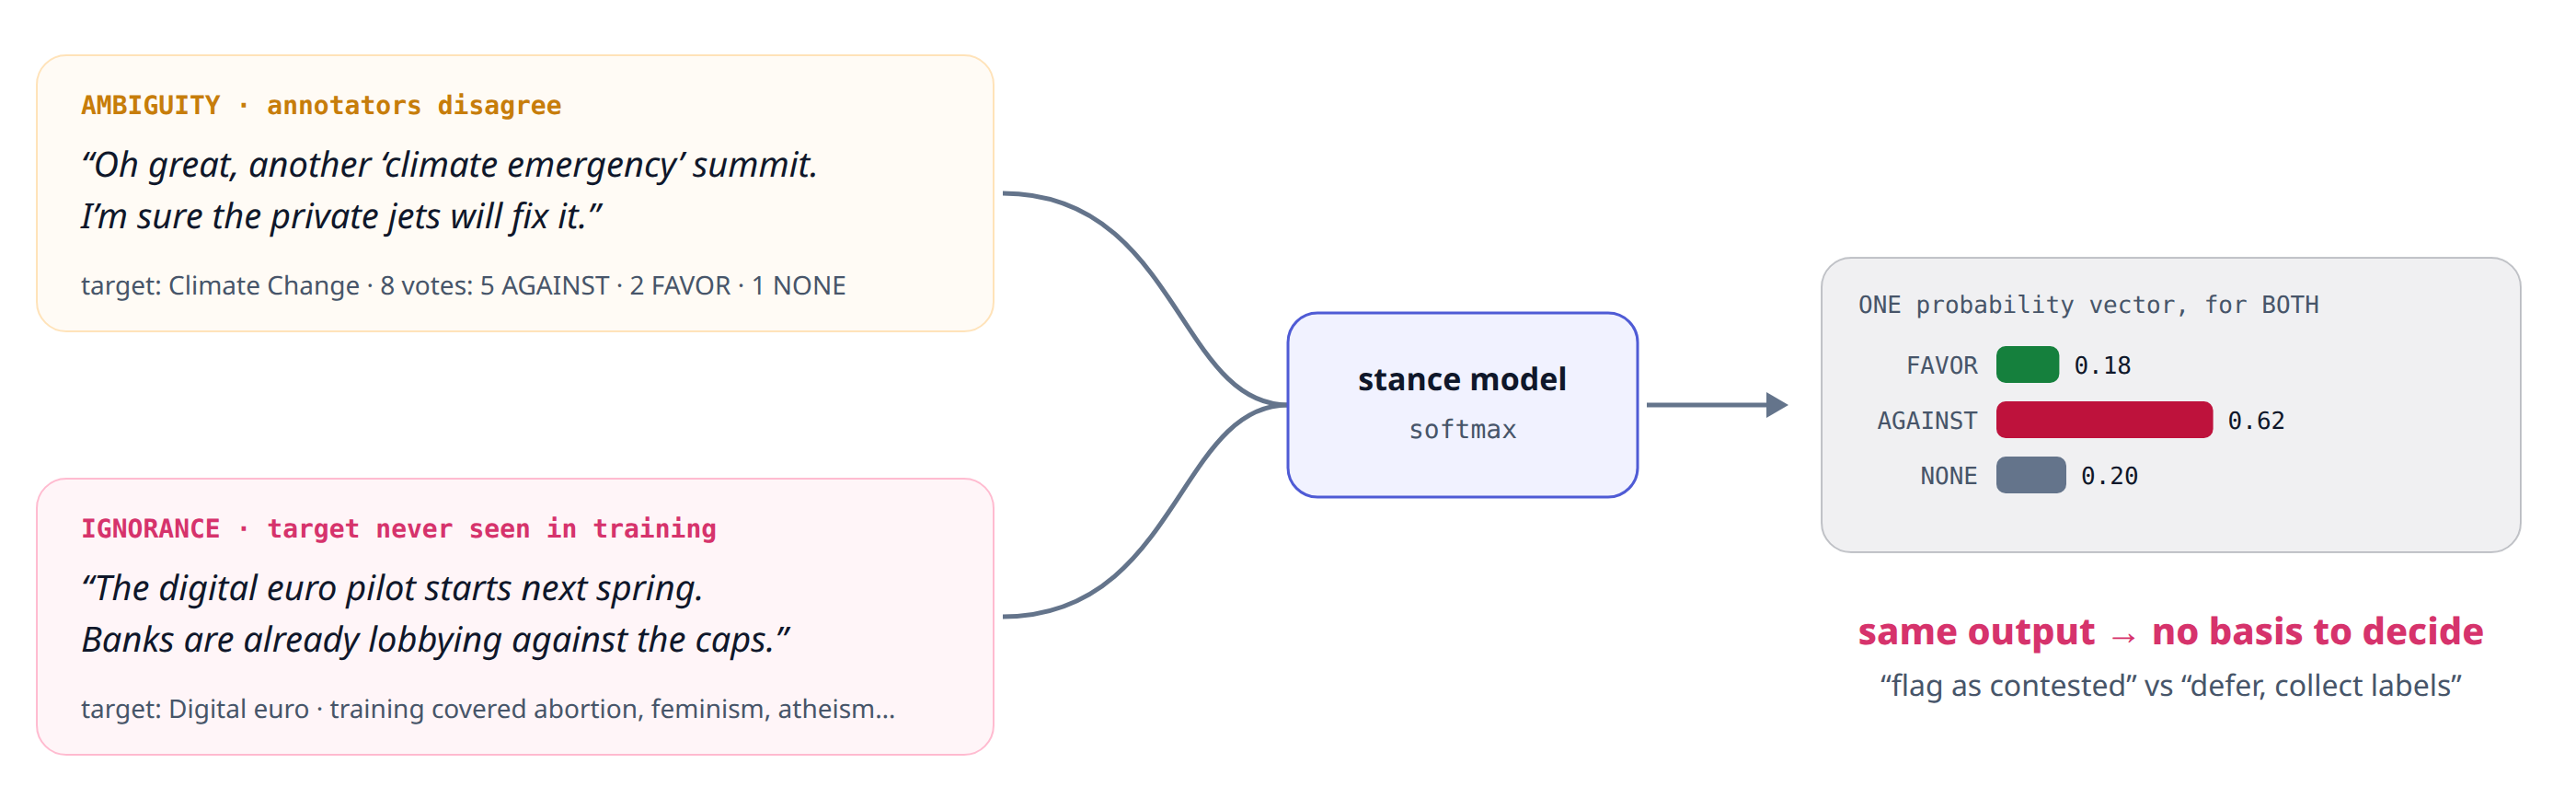
\includegraphics[width=\textwidth]{results/fig/arch/same_vector.png}
\caption{Two very different situations, one identical softmax output. Neither ``flag as contested'' nor ``defer and collect labels'' can be justified from the vector alone.}
\label{fig:samevec}
\end{figure}

\subsection{Problem statement}
\begin{quote}
Existing stance detectors output a single distribution $p(y\mid x,t)$ that conflates aleatoric and epistemic uncertainty; consequently they are over-confident on unseen targets and cannot justify abstention. We seek a detector that outputs a \emph{credal set} $\credal(x,t)\subseteq\Delta_3$, represented by class-wise lower and upper probabilities $[\lo{P}(y),\up{P}(y)]$, such that (a) the set's \emph{location} reflects ambiguity and its \emph{size} reflects ignorance, (b) the set can be calibrated to cover the true human label distribution with a distribution-free guarantee, and (c) the set supports a predict / set-valued / defer decision. The method must need \textbf{no new annotation}, run on one GPU, and be evaluated on in-target, cross-target and cross-dataset stance data.
\end{quote}

\subsection{Research questions and hypotheses}
\begin{description}[leftmargin=1.4cm,style=nextline]
\item[RQ1] Do credal stance models give better uncertainty estimates than softmax, temperature scaling, MC-dropout, deep ensembles and evidential deep learning at equal accuracy? \emph{H1:} better calibration and selective risk at $\pm1$ pt macro-F1.
\item[RQ2] Does the credal decomposition separate ambiguity from ignorance? \emph{H2:} the epistemic score rises on unseen targets; the aleatoric score tracks human label entropy.
\item[RQ3] Can credal sets be calibrated to cover the human label distribution? \emph{H3:} conformal credal sets attain $1-\alpha$ coverage; soft-label-trained sets are more efficient.
\item[RQ4] Does credal uncertainty improve decisions? \emph{H4:} lower expected cost than confidence thresholding at every deferral budget.
\item[RQ5] Do LLM prompt-ensemble credal sets beat single-prompt LLM confidence? \emph{H5:} lower ECE, higher error-detection AUROC.
\end{description}

% =====================================================================
\section{Background}
% =====================================================================

\subsection{Credal sets and the two kinds of uncertainty}
A credal set is a closed convex set $\credal\subseteq\simplex$ of candidate distributions for an imprecisely known ground truth \cite{walley1991}. We use probability-interval credal sets
\begin{equation}
\credal(l,u)=\{p\in\simplex:\ l_k\le p_k\le u_k\ \forall k\}.
\end{equation}
With Shannon entropy $H$ in bits, the standard measures are \cite{abellan2006,hullermeier2021}
\begin{equation}
\TU=\up{H}=\max_{p\in\credal}H(p),\qquad \AU=\lo{H}=\min_{p\in\credal}H(p),\qquad \EU=\up{H}-\lo{H}.
\label{eq:dec}
\end{equation}
A \emph{small} set around a spread-out distribution is ``confident that the text is ambiguous'' (high AU, low EU); a \emph{large} set is ``do not know which distribution is right'' (high EU); Figures~\ref{fig:credalintro}--\ref{fig:decomp}. Sale et al.\ \cite{sale2023} show that the set's volume is a sound epistemic measure only for binary problems; Gonzalez-Garcia et al.\ \cite{gonzalez2026} propose distance-based multiclass measures, of which the interval width $\sum_k(u_k-l_k)$ is the simplest proxy. We report both the entropy decomposition and the width.

\begin{figure}[t]
\centering
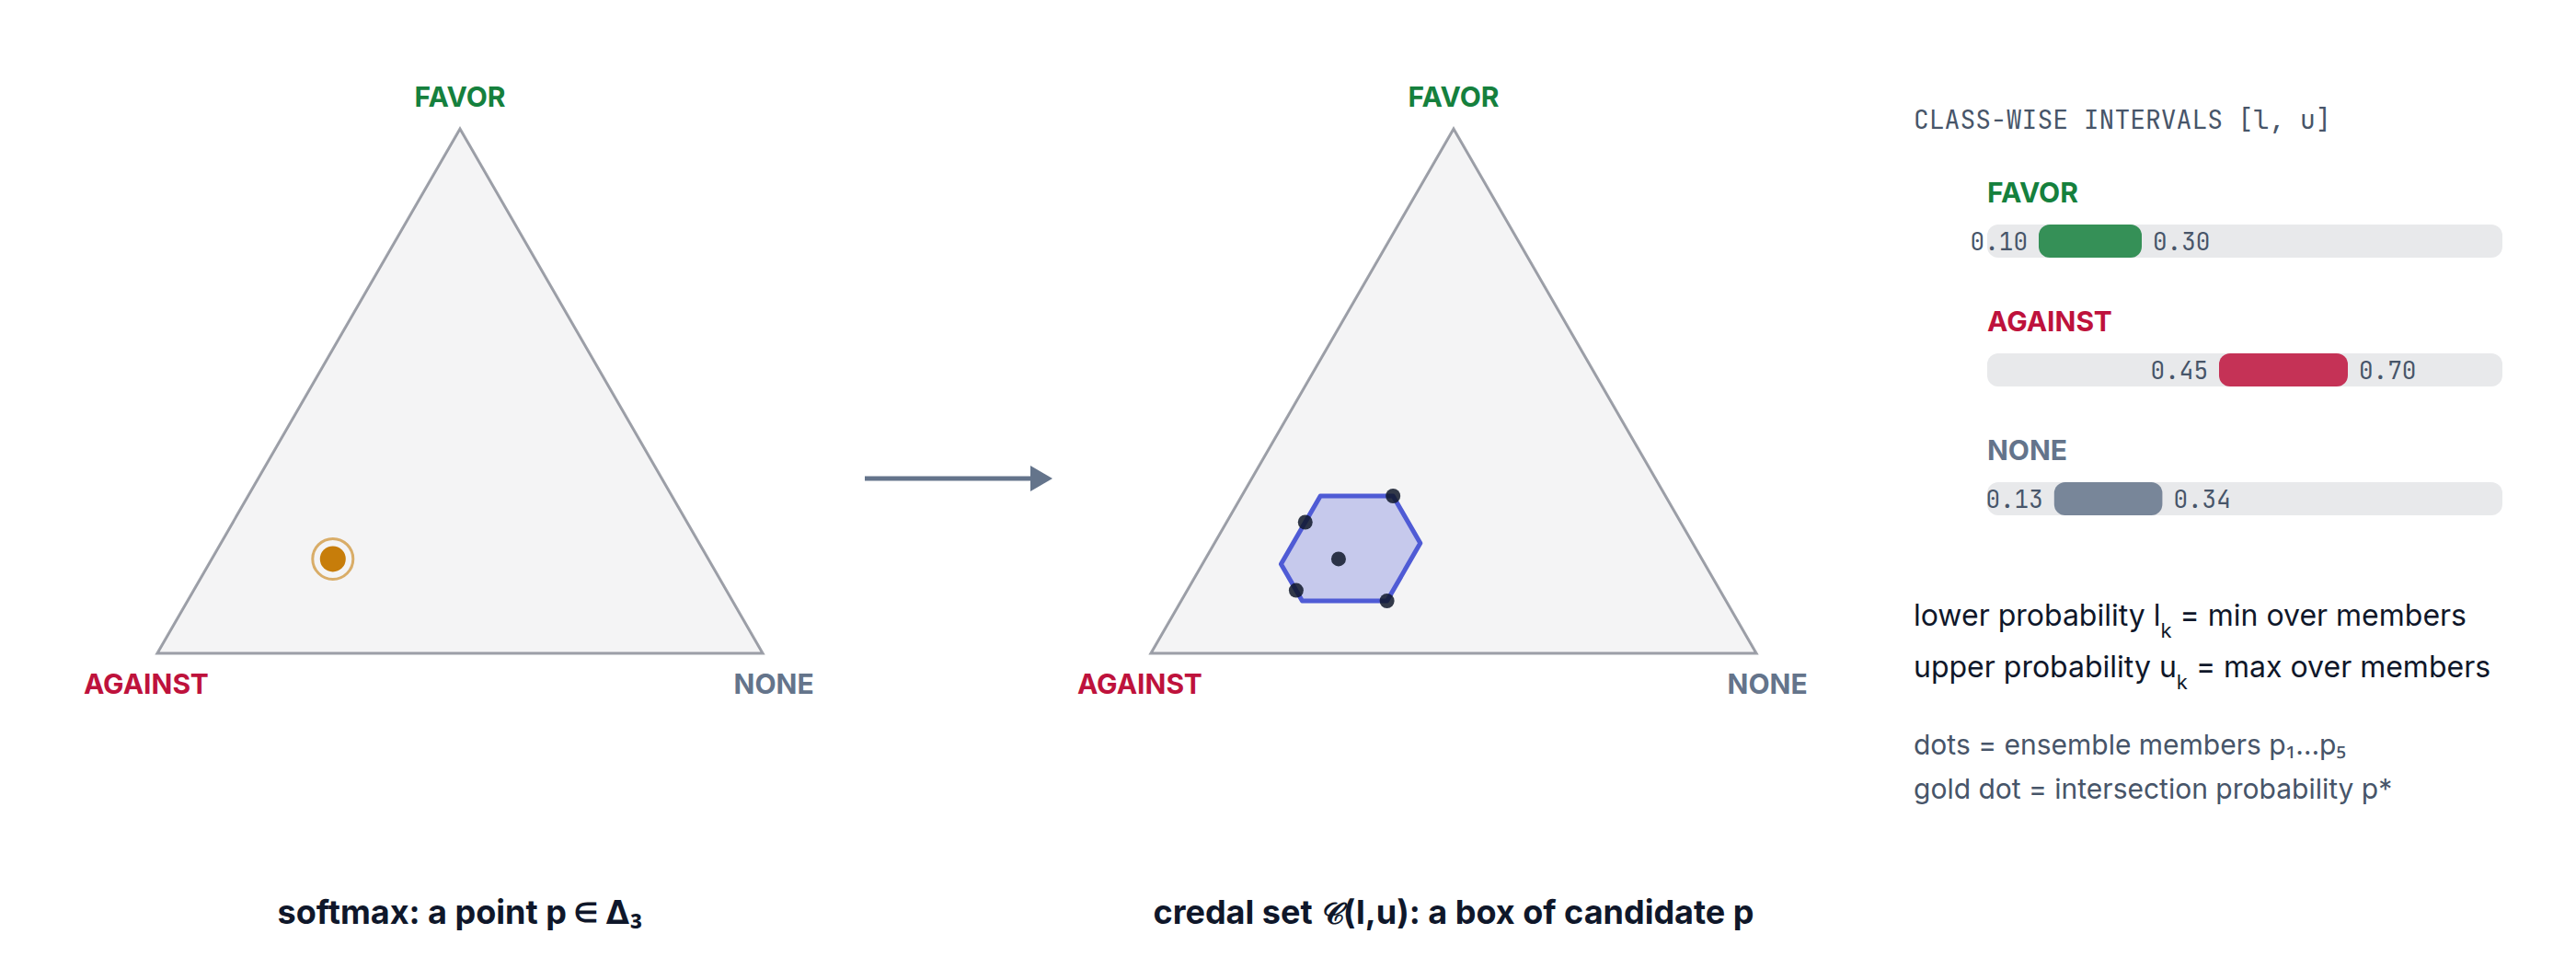
\includegraphics[width=\textwidth]{results/fig/arch/credal_intro.png}
\caption{From a point to a set. Left: softmax returns one point on the stance simplex. Right: the ensemble members (dots) span a probability-interval credal set whose class-wise bounds $l_k=\min_m p_{m,k}$, $u_k=\max_m p_{m,k}$ are shown on the far right; the gold dot is the intersection probability $p^*$.}
\label{fig:credalintro}
\end{figure}
\begin{figure}[t]
\centering
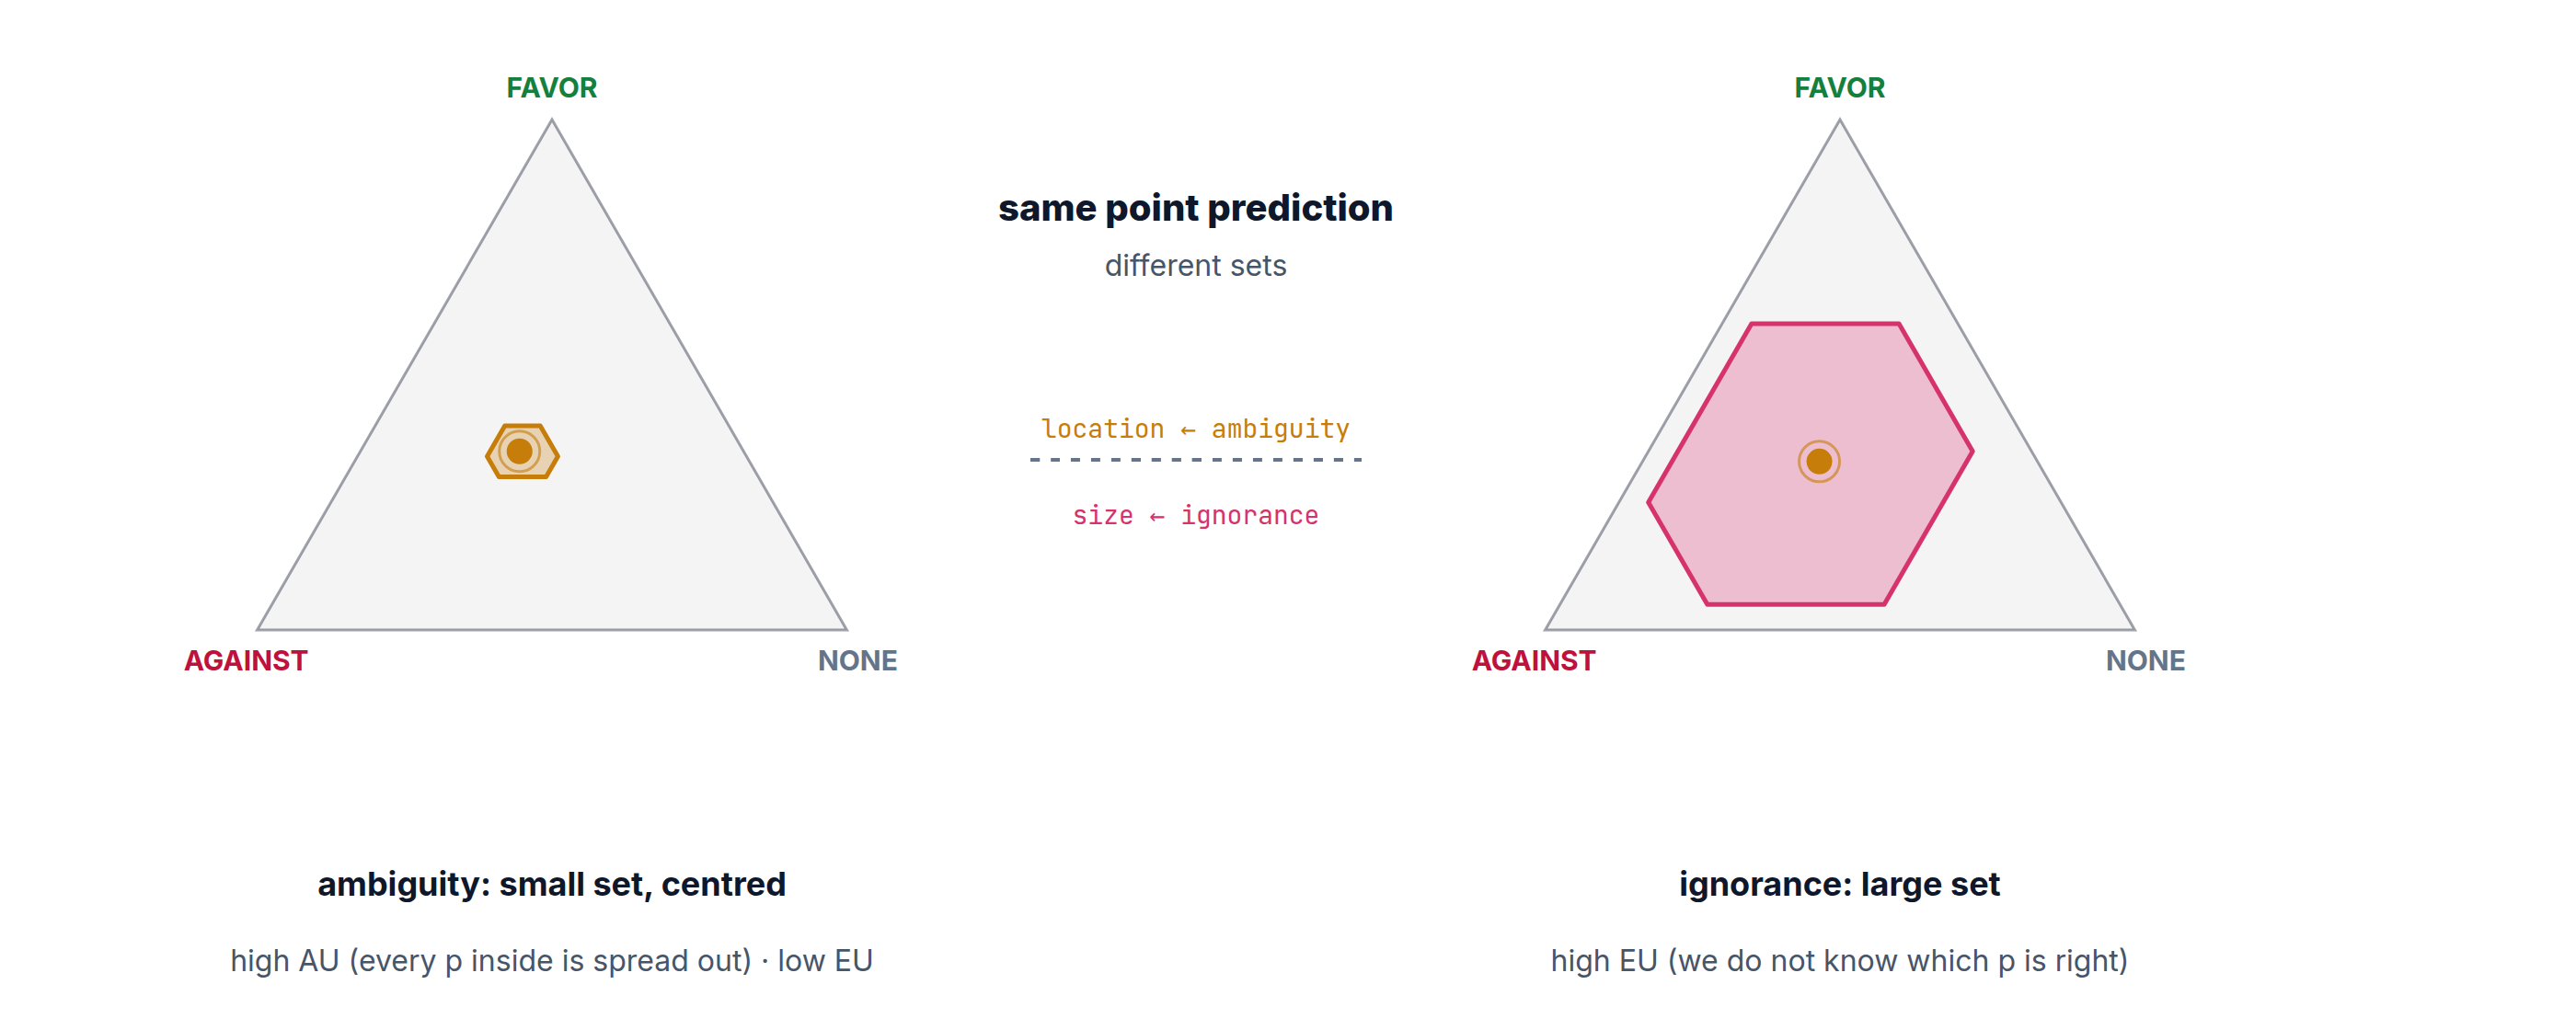
\includegraphics[width=0.92\textwidth]{results/fig/arch/ambiguity_vs_ignorance.png}
\caption{Location encodes ambiguity, size encodes ignorance. Both sets share the same point prediction. Left: a small set near the centre, the model is confident that the item is contested (high AU, low EU). Right: a large set, the model does not know which distribution is right (high EU).}
\label{fig:simplex}
\end{figure}
\begin{figure}[t]
\centering
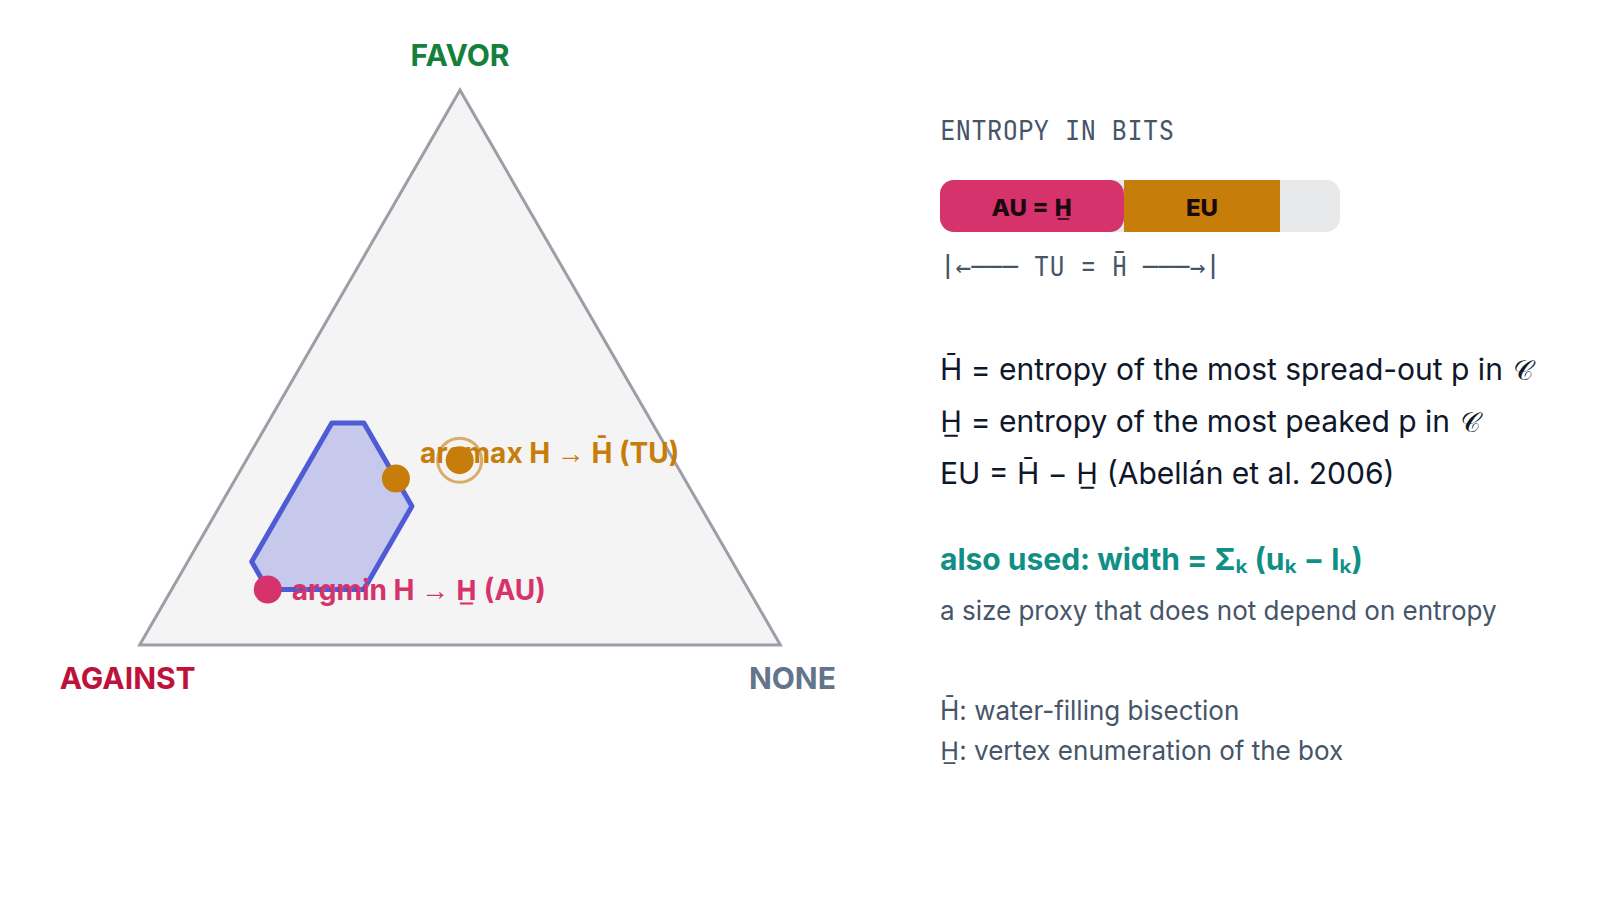
\includegraphics[width=0.7\textwidth]{results/fig/arch/decomposition.png}
\caption{Measuring a credal set. $\up H$ is attained by the most spread-out distribution in the set, $\lo H$ by the most peaked one; $\EU=\up H-\lo H$. The interval width $\sum_k(u_k-l_k)$ is an entropy-free size proxy.}
\label{fig:decomp}
\end{figure}

\subsection{Classical versus modern credal models}
The claim that ``credal networks only work on tabular data'' is true of classical credal networks \cite{cozman2000} and the naive credal classifier \cite{corani2008}, which place imprecise probability tables inside a graphical model over few discrete variables. Modern credal deep learning places the credal set \emph{at the output} of a neural network \cite{wang2025wrapper,wang2024crede,wang2025creinn,javanmardi2024,lohr2025,hofman2026,credro2026,manchingal2026}; the encoder handles the raw text. Credal sets have been evaluated on ChaosNLI, an NLI benchmark with $\sim$100 annotators per item \cite{javanmardi2024,hofman2026}, and on LLMs via LoRA ensembles \cite{manchingal2026}. Stance detection has the same structure as NLI (a text pair, three classes, high human disagreement); EZ-Stance even reformulates zero-shot stance as NLI \cite{zhao2024}. Figure~\ref{fig:classical} contrasts the two families.

\begin{figure}[t]
\centering
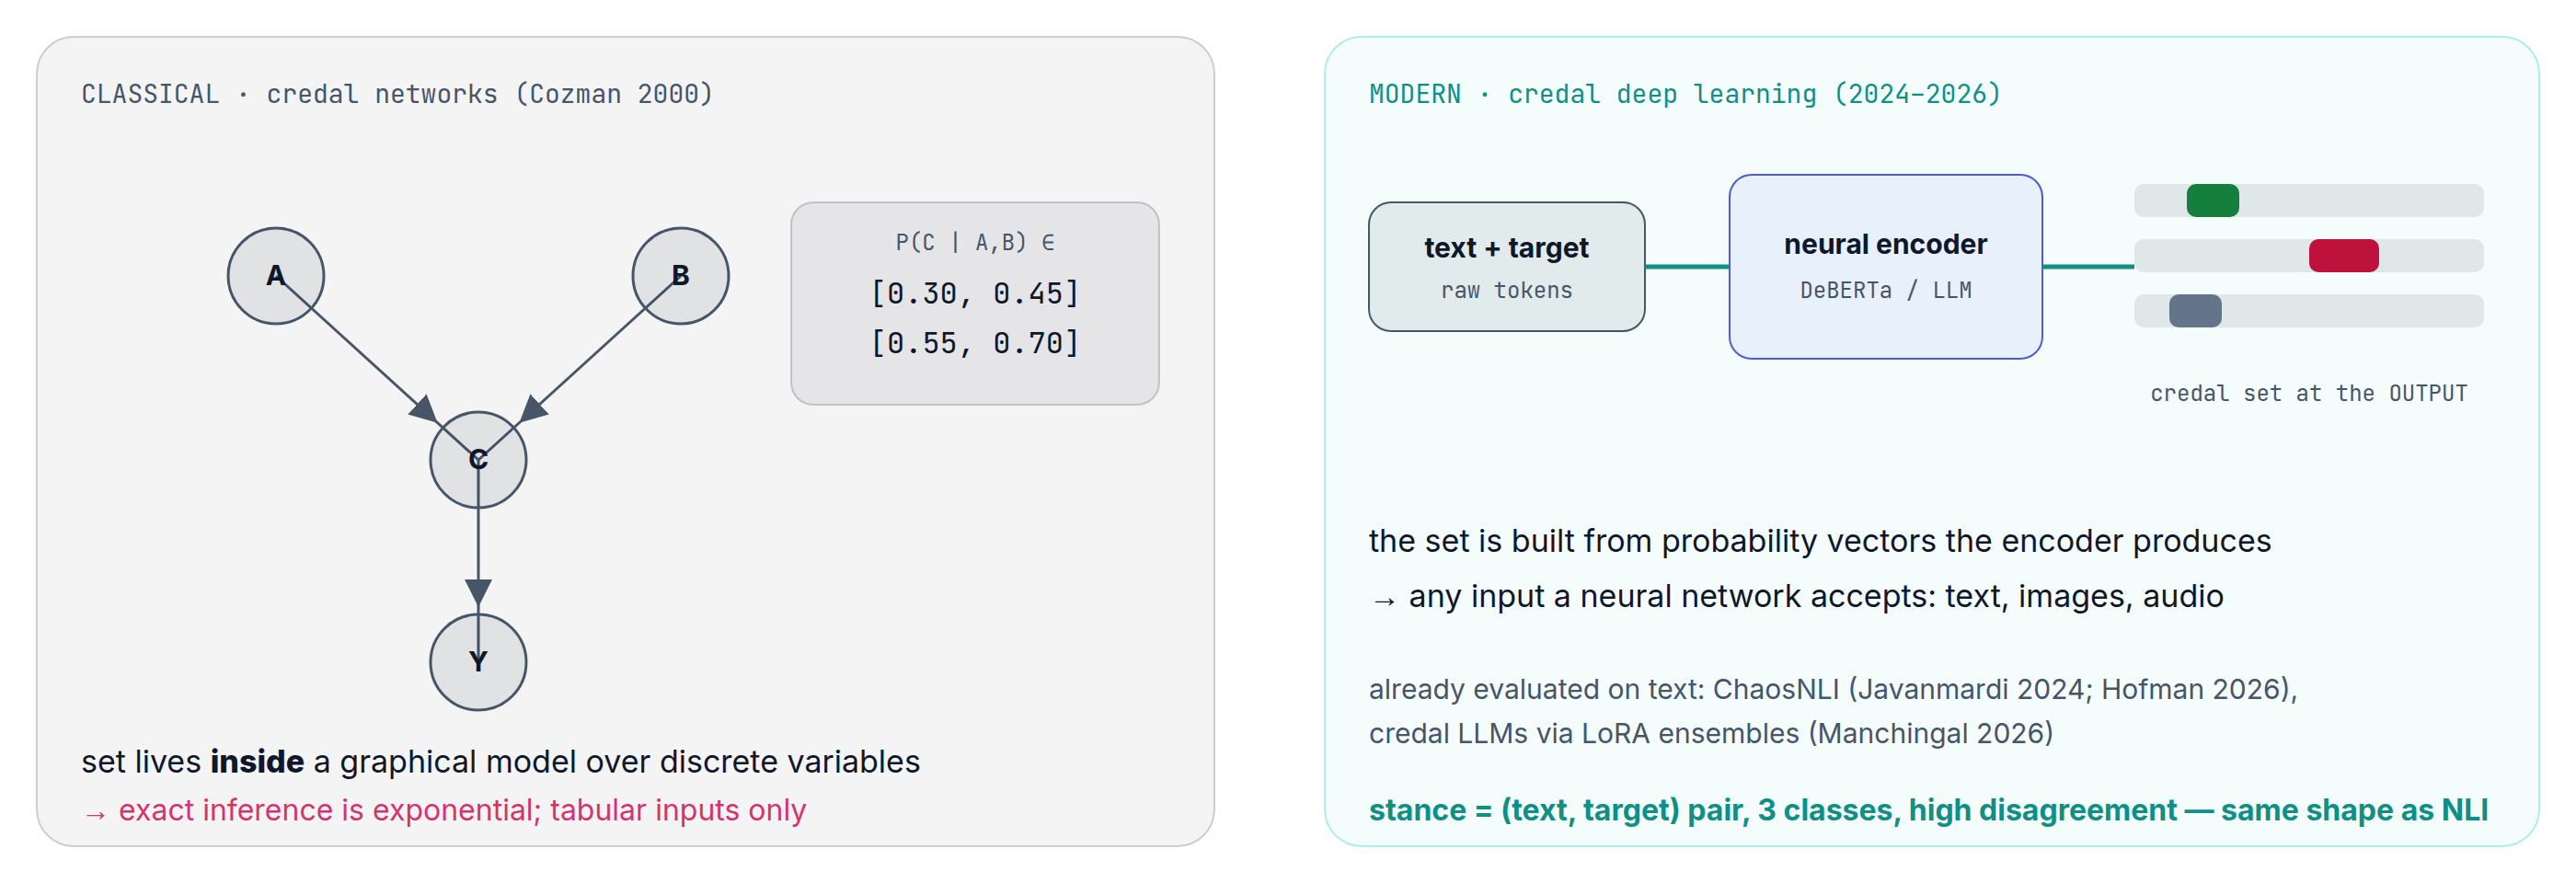
\includegraphics[width=\textwidth]{results/fig/arch/classical_vs_modern.png}
\caption{Classical credal networks keep imprecise probability tables inside a graphical model over discrete variables, which restricts them to tabular inputs and exponential exact inference. Modern credal deep learning builds the set from the probability vectors a neural encoder produces, so raw text is handled by the encoder.}
\label{fig:classical}
\end{figure}

% =====================================================================
\section{Alternative Credal Architectures Considered}
% =====================================================================

All constructions share one backbone (DeBERTa-v3-base \cite{he2023}, $[\mathrm{CLS}]$ pooling, linear head) so that only the credal construction differs.

\paragraph{A1. Post-hoc credal wrapper over a deep ensemble (CreWrap-DE) \cite{wang2025wrapper}.}
Train $M$ standard members (seed + 80\% bootstrap); $l_k=\min_m p_{m,k}$, $u_k=\max_m p_{m,k}$. Point prediction by the intersection probability
\begin{equation}
p^*_k=l_k+\alpha(u_k-l_k),\qquad \alpha=\frac{1-\sum_k l_k}{\sum_k(u_k-l_k)}.
\label{eq:ip}
\end{equation}
Same members as the Bayesian deep-ensemble baseline (DE-MI) \cite{lakshminarayanan2017}, so the comparison isolates the credal representation.

\paragraph{A2. Credal wrapper over MC-dropout (MCD-Credal).} One model, $T=10$ dropout samples \cite{gal2016}, same wrapper.

\paragraph{A3. Credal Deep Ensembles (CreDE) \cite{wang2024crede}.}
Each member has an interval head: midpoint $m$ and half-length $h=\mathrm{softplus}(\cdot)$ give $[a_L,a_U]=[m-h,m+h]$, mapped to probability intervals by the interval softmax, written here in its numerically stable form
\begin{equation}
q_{L,i}=\sigma\!\big(a_{L,i}-\mathrm{LSE}_{k\ne i}\,m_k\big),\qquad q_{U,i}=\sigma\!\big(a_{U,i}-\mathrm{LSE}_{k\ne i}\,m_k\big),
\end{equation}
which satisfies $q_L\le q_U$ and $\sum q_L\le1\le\sum q_U$. Loss $=\mathrm{CE}(q_U)+\mathrm{CE}(q_L)$ on the hardest $\delta=0.5$ fraction of each batch. The ensemble averages the members' reachable intervals.

\paragraph{A4. Distributionally robust credal ensembles (CreDRO) \cite{credro2026}.}
Members are ordinary networks that differ only in a CVaR-DRO fraction $\delta_i$: each batch is sorted by per-sample loss and only the top $\lfloor\delta_i B\rfloor$ samples receive gradient; $\delta_i$ is spread uniformly over $[0.5,1]$. Credal set by min/max as in A1. Same cost as a deep ensemble, but members disagree \emph{by design} on the hard, shifted part of the data.

\paragraph{A5. Single-model credal sets by decalibration (EffCre) \cite{hofman2026,lohr2025}.}
From one trained model, shift the logits by $t\,e_k$ and keep every $t$ whose log-likelihood on a reference set stays within $\log\alpha$ of the maximum; bounds are $p_k(x;t_k^{\pm})$ found by bisection. We use the held-out calibration split as reference (a fine-tuned transformer fits its training set almost perfectly) and sweep $\alpha\in\{0.5,10^{-2},10^{-4},10^{-6}\}$.

\paragraph{A6. Prompt-paraphrase credal sets from an LLM (Prompt-Credal) \cite{manchingal2026,xiong2024}.}
Zero-shot Qwen2.5-3B-Instruct with 8 system/instruction paraphrases; class probabilities from the softmax restricted to the verbalizer tokens \emph{favor/against/none}; credal set by min/max over prompts. Baselines: a single prompt, and the prompt mixture (mean + mutual information).

\subsection{Proposed: human-distribution-supervised robust credal ensemble (CreDRO-Soft)}
Two deficiencies motivate the proposal. First, A1--A5 are trained on \textbf{hard labels}: nothing in the training signal says how \emph{contested} an item is, so the lower entropy of the resulting credal set is an artefact of the backbone rather than a model of human disagreement. Second, seed/bootstrap diversity is incidental: members disagree where they happen to, not where the data is shifted.

CreDRO-Soft trains CreDRO members against the \textbf{empirical human label distribution} $\lambda_x$ wherever per-annotator votes exist (SemEval released $\approx8$ votes per tweet), i.e.\ the per-sample loss is $-\sum_k\lambda_{x,k}\log p_k$, and keeps the CVaR-DRO member diversity. The intended division of labour is: \emph{location} of the credal set $\leftarrow$ human disagreement (every member is pulled towards $\lambda_x$, so $\lo{H}$ tracks human entropy); \emph{size} of the credal set $\leftarrow$ distributional robustness (members with small $\delta$ concentrate on the hardest tail, members with $\delta=1$ fit everything; they diverge most on items unlike the training distribution). The two ingredients are also evaluated separately (CreWrap-Soft, CreDRO), giving a $2\times2$ ablation. Figure~\ref{fig:credrosoft} summarises the construction.

\begin{figure}[t]
\centering
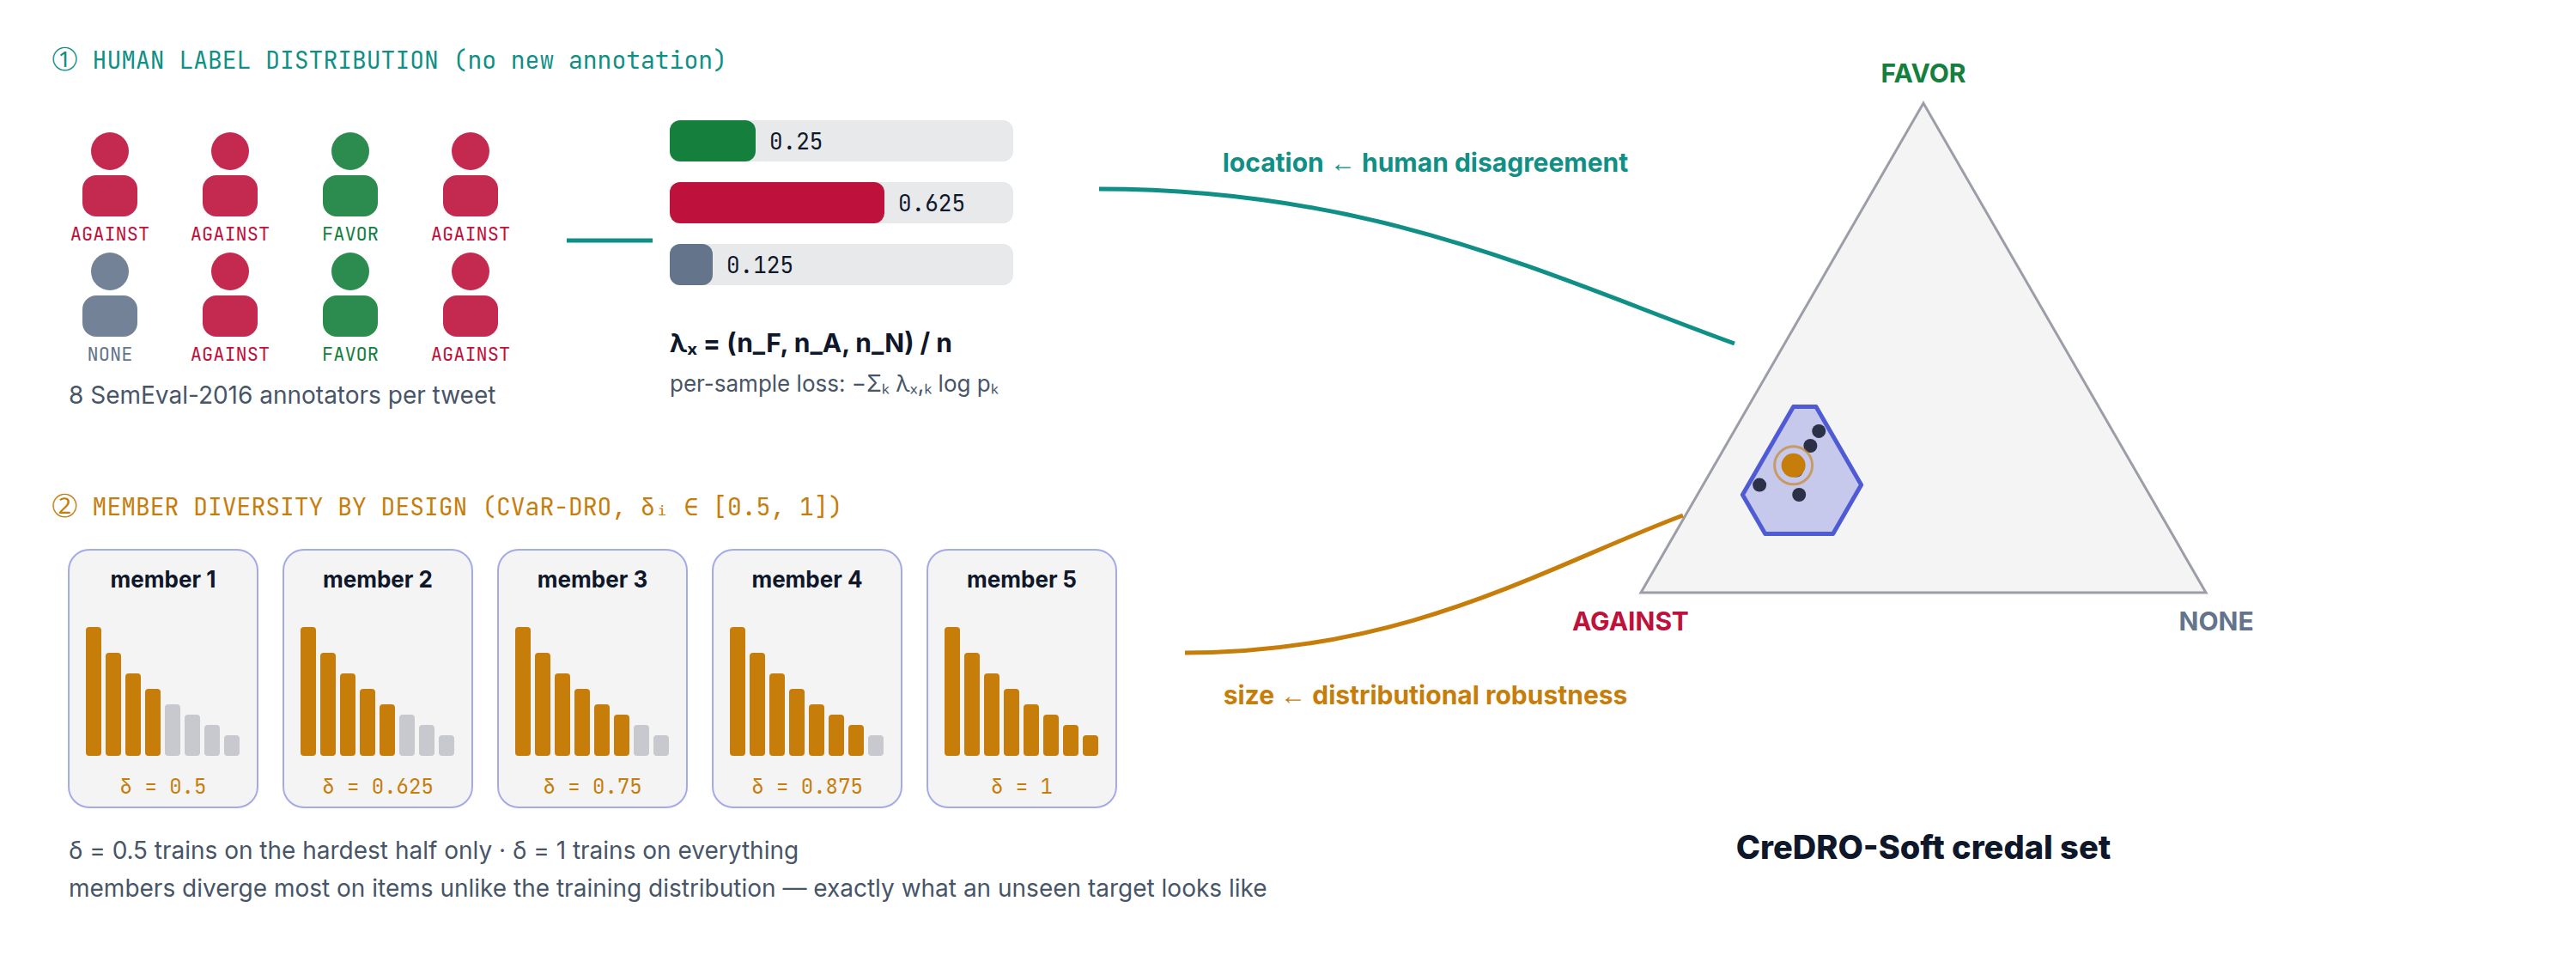
\includegraphics[width=\textwidth]{results/fig/arch/credro_soft.png}
\caption{CreDRO-Soft. (1) Released per-annotator votes become a human label distribution $\lambda_x$ that every member is trained towards; this sets the \emph{location} of the credal set. (2) Members differ only in the CVaR-DRO fraction $\delta_i$ of each batch that receives gradient; this sets the \emph{size} of the set, because members diverge most on items unlike the training distribution.}
\label{fig:credrosoft}
\end{figure}

\subsection{Calibration and decision layers (shared)}
\textbf{Conformal credal calibration} \cite{javanmardi2024,angelopoulos2023}: non-conformity $s_i=\TV(\lambda_i,g(x_i))=\tfrac12\sum_k|\lambda_{i,k}-g_k(x_i)|$ on the held-out calibration split, quantile $\hat q$ at level $1-\alpha$, calibrated set $\{\lambda:\TV(\lambda,g(x))\le\hat q\}$ with bounds $[g_k-\hat q,\,g_k+\hat q]$; $P(\lambda_x\in\hat\credal(x))\ge1-\alpha$ under exchangeability. We add a \emph{credal-dilation} variant whose score is the distance of $\lambda$ to the predicted box (zero if inside).
\textbf{Interval dominance} \cite{troffaes2007}: $\ND(x)=\{k:u_k\ge\max_j l_j\}$; one non-dominated class $\to$ predict; several and low EU $\to$ set-valued answer; high EU $\to$ defer (Figure~\ref{fig:decision}).

\begin{figure}[t]
\centering
\begin{minipage}[c]{0.40\textwidth}\centering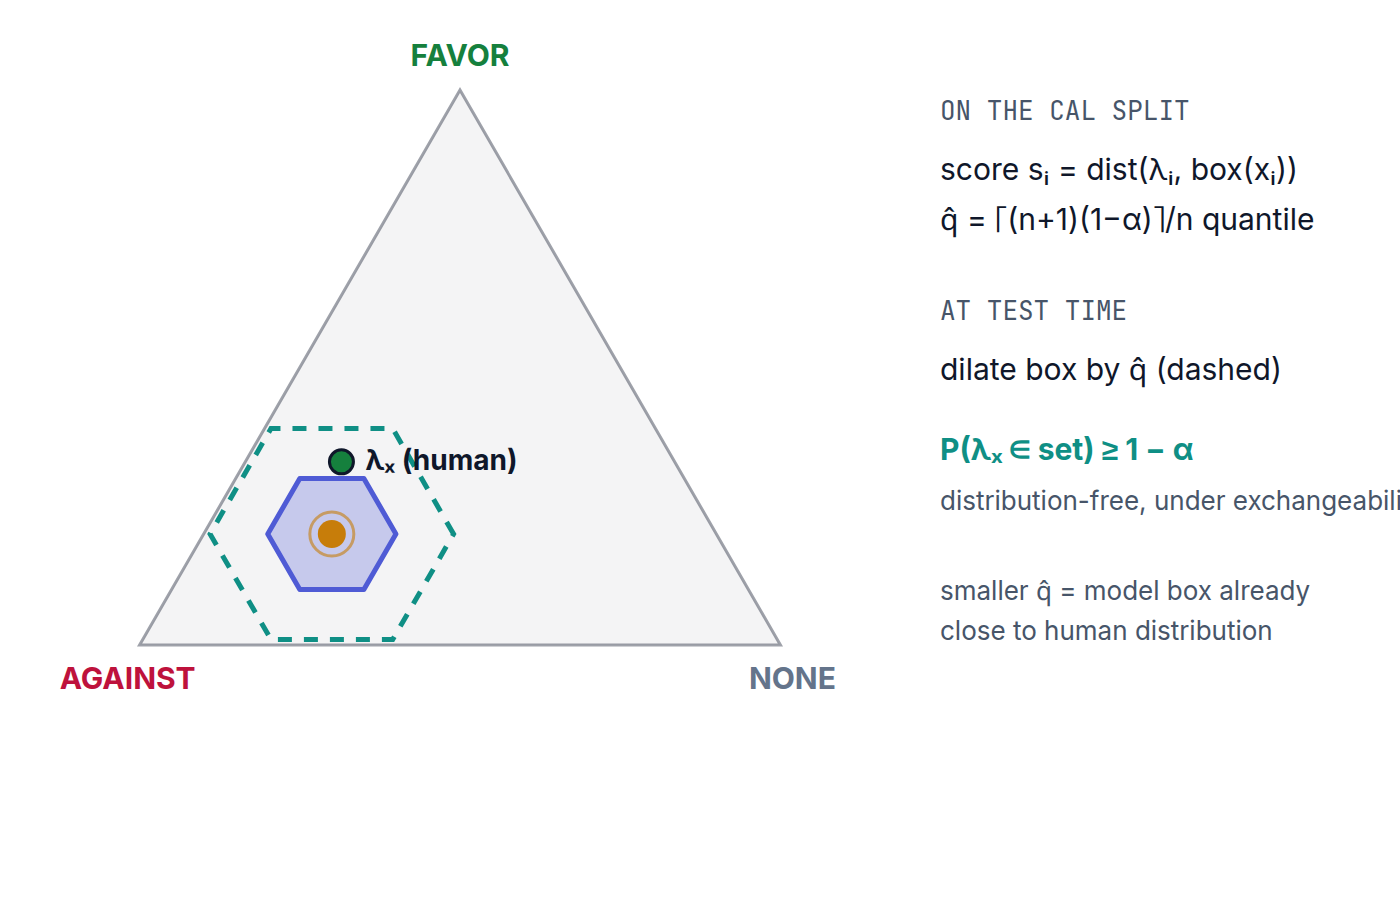
\includegraphics[width=\textwidth]{results/fig/arch/conformal.png}\end{minipage}\hfill
\begin{minipage}[c]{0.57\textwidth}\centering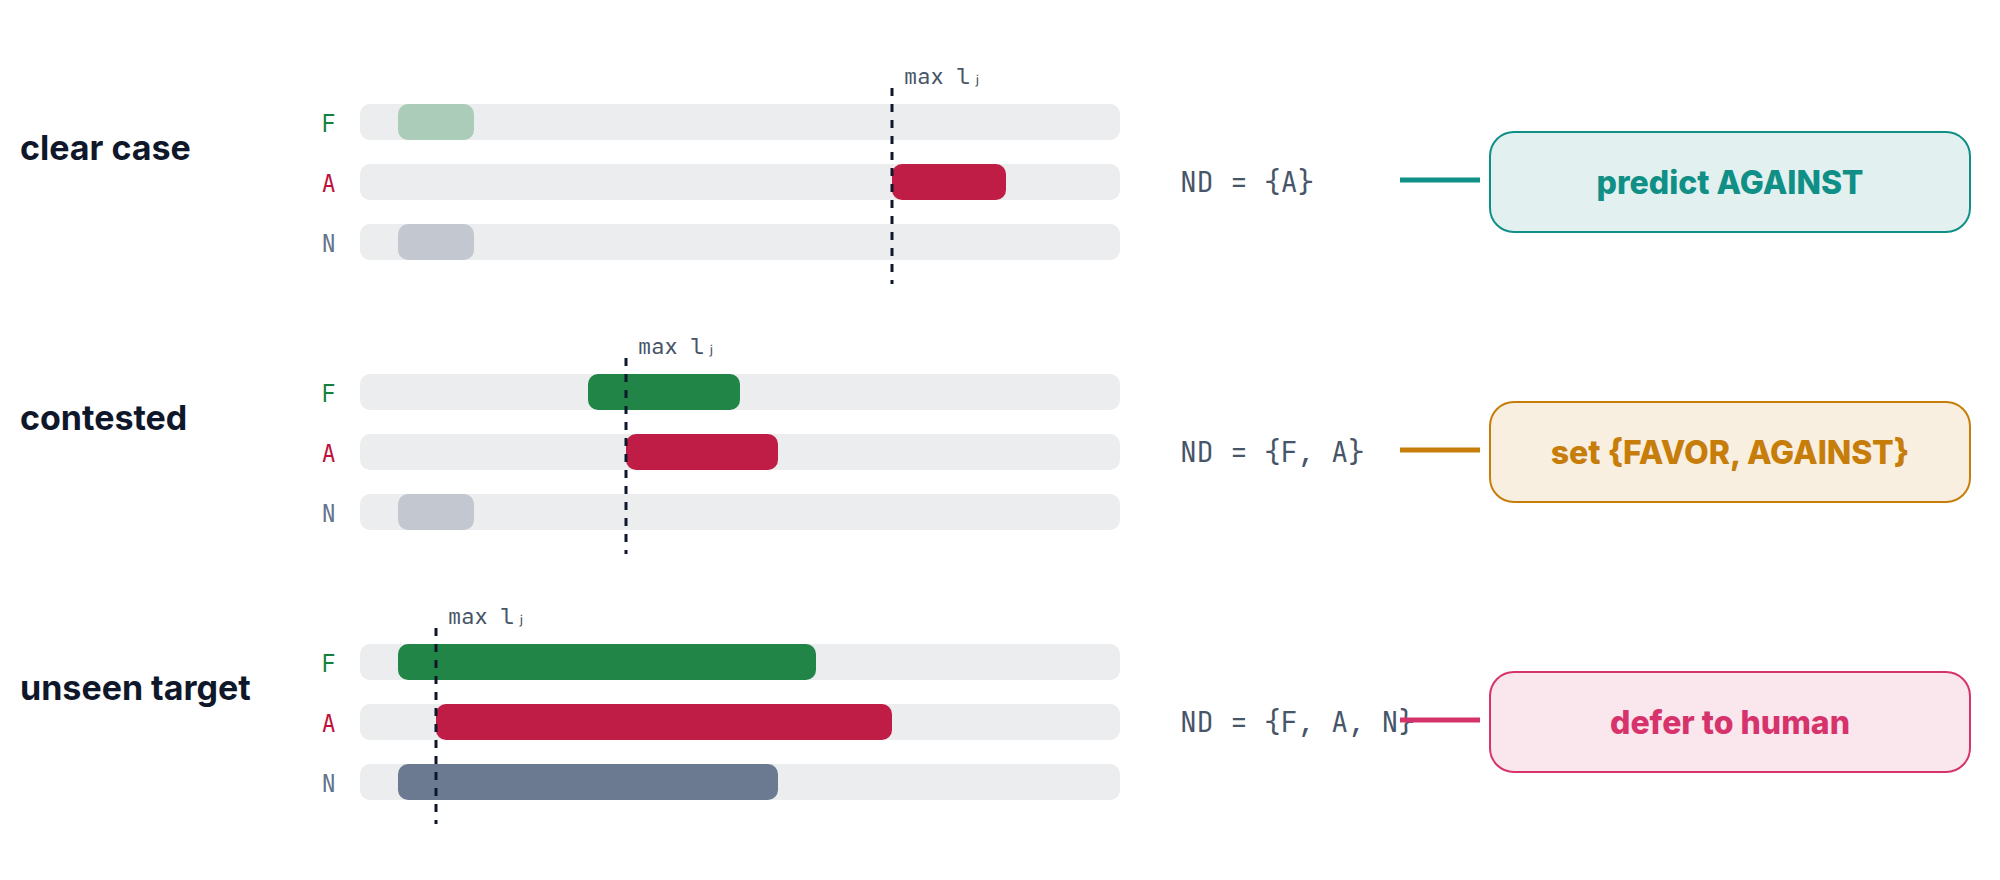
\includegraphics[width=\textwidth]{results/fig/arch/dominance.png}\end{minipage}
\caption{Left: conformal credal calibration by box dilation. The score of a calibration item is the distance of its $\lambda$ to the predicted box; the $(1-\alpha)$ quantile $\hat q$ dilates the box at test time (dashed), giving $P(\lambda_x\in\hat\credal(x))\ge1-\alpha$ under exchangeability. Right: interval dominance. A class is non-dominated when its upper probability reaches the largest lower probability (dashed line); one class $\to$ predict, several with low EU $\to$ set-valued answer, several with high EU $\to$ defer.}
\label{fig:decision}
\end{figure}

% =====================================================================
\section{System Architecture}
% =====================================================================

\begin{figure}[t]
\centering
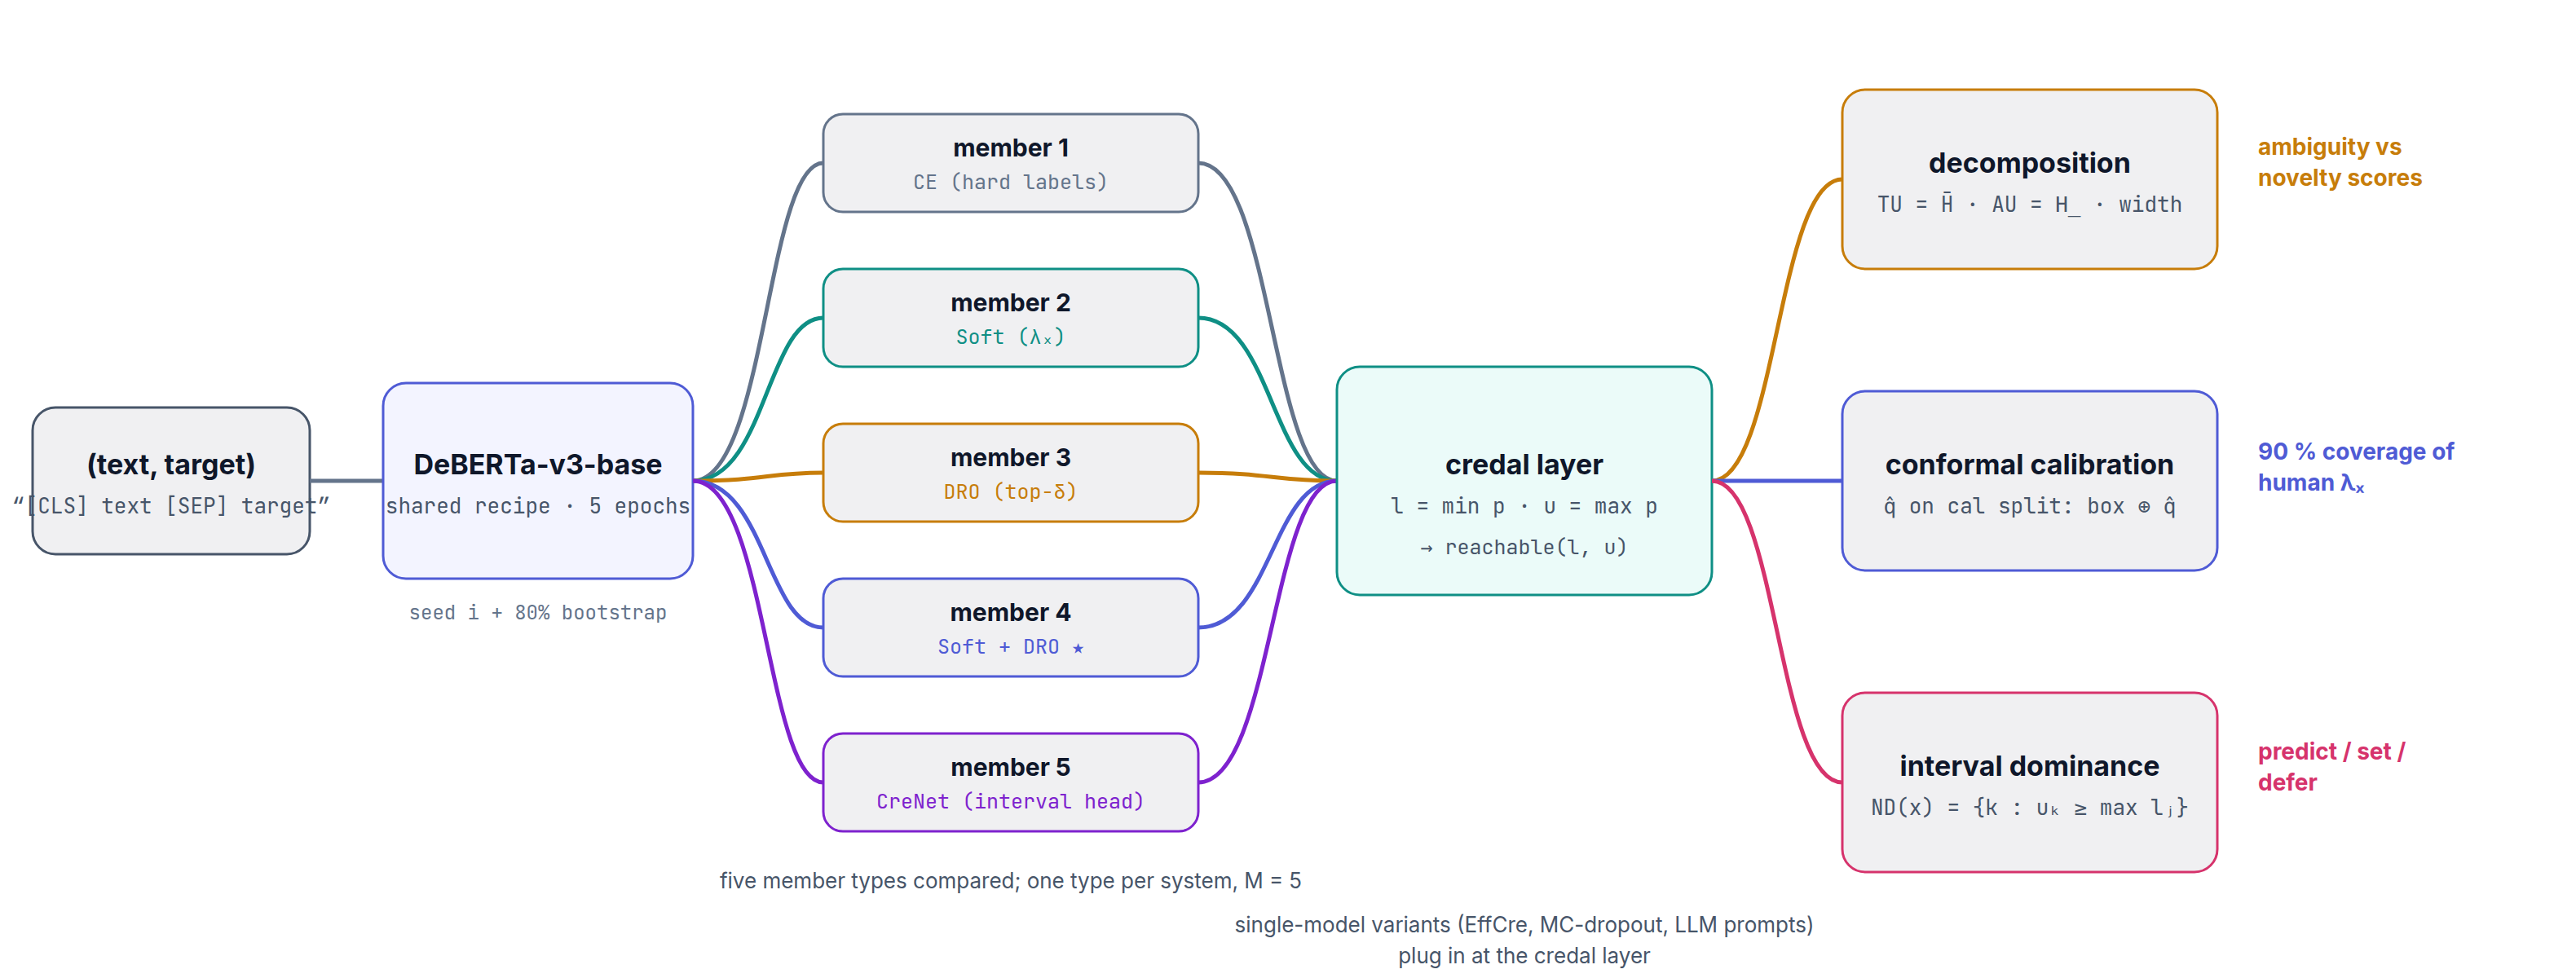
\includegraphics[width=\textwidth]{results/fig/arch/pipeline.png}
\caption{System architecture. A (text, target) pair is encoded by DeBERTa-v3-base; $M$ members trained with one of five objectives produce probability vectors; the credal layer takes their class-wise min and max and tightens the bounds to the reachable set; three consumers read the set: the uncertainty decomposition, conformal calibration against the human label distributions of the calibration split, and interval dominance for the predict / set / defer decision. Single-model variants (EffCre, MCD-Credal) and the LLM prompt-credal plug in at the credal layer.}
\label{fig:arch}
\end{figure}
\begin{figure}[t]
\centering
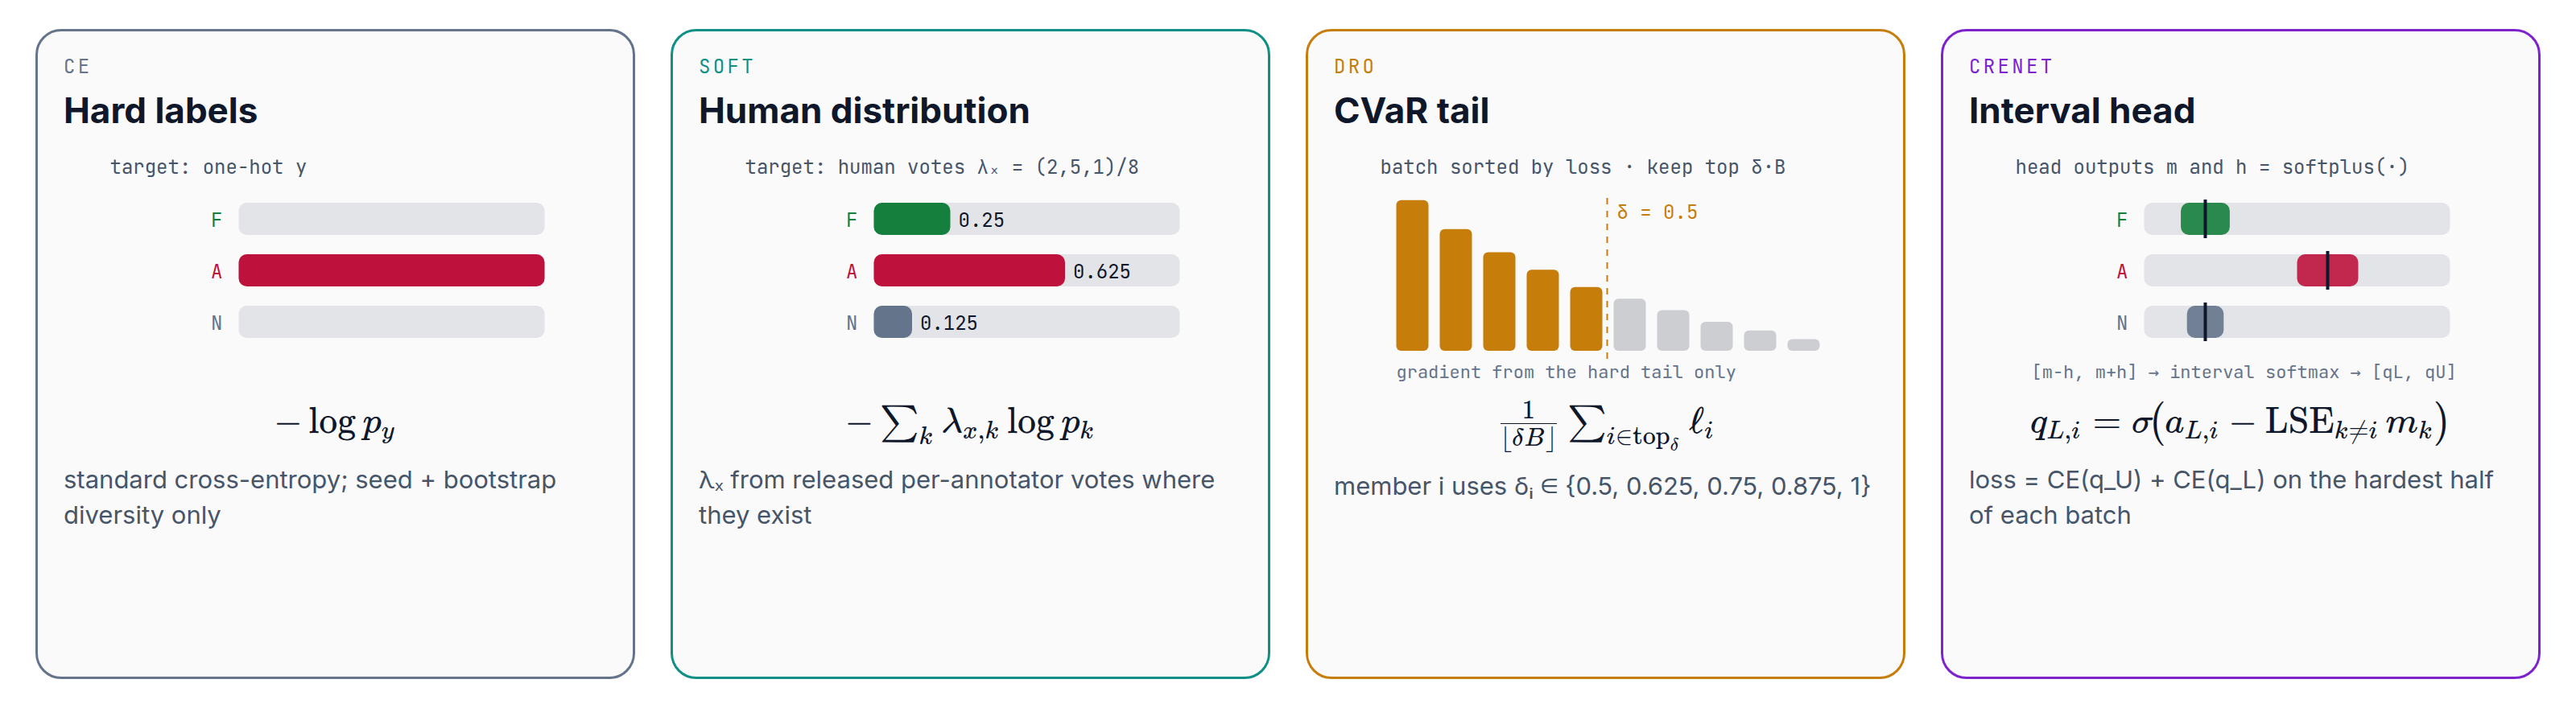
\includegraphics[width=\textwidth]{results/fig/arch/members.png}
\caption{The four member objectives. Hard-label cross-entropy; soft cross-entropy against the human vote distribution; the CVaR-DRO loss that back-propagates only the hardest $\delta$ fraction of each batch; and the interval head of Credal Deep Ensembles with its interval softmax. Every system in the study is one member type wrapped by the same credal layer.}
\label{fig:members}
\end{figure}

% =====================================================================
\section{Data and Experimental Protocol}
% =====================================================================

\begin{table}[h]
\centering\small
\begin{tabular}{p{6.2cm} r r p{5.2cm}}
\toprule
Split & Items & With votes & Role \\
\midrule
SemEval-2016 train (80\%) & 2{,}250 & 1{,}934 & member training \\
SemEval-2016 cal (20\% of train, stratified by target; never trained on) & 564 & 485 & temperature, EffCre reference, conformal calibration \\
SemEval-2016 test (official) \cite{mohammad2016} & 1{,}249 & 1{,}080 & in-target evaluation; human alignment \\
SemEval low-agreement pool (dropped from the task) \cite{mohammad2017} & 1{,}385 (1{,}101 on seen targets) & 1{,}385 & ambiguity stress test \\
P-Stance test (Trump, Biden, Sanders; binary) \cite{li2021} & 2{,}157 & -- & cross-dataset unseen targets \\
COVID-19-Stance test (4 targets) \cite{glandt2021} & 800 & -- & cross-dataset unseen targets \\
\bottomrule
\end{tabular}
\caption{Data. $\lambda_x=(n_{\textsc{favor}},n_{\textsc{against}},n_{\textsc{none}})/n$, median $n=8$; \textsc{neutral} votes mapped to \textsc{none}. The \emph{Climate Change} target has no released votes.}
\label{tab:data}
\end{table}

\begin{figure}[t]
\centering
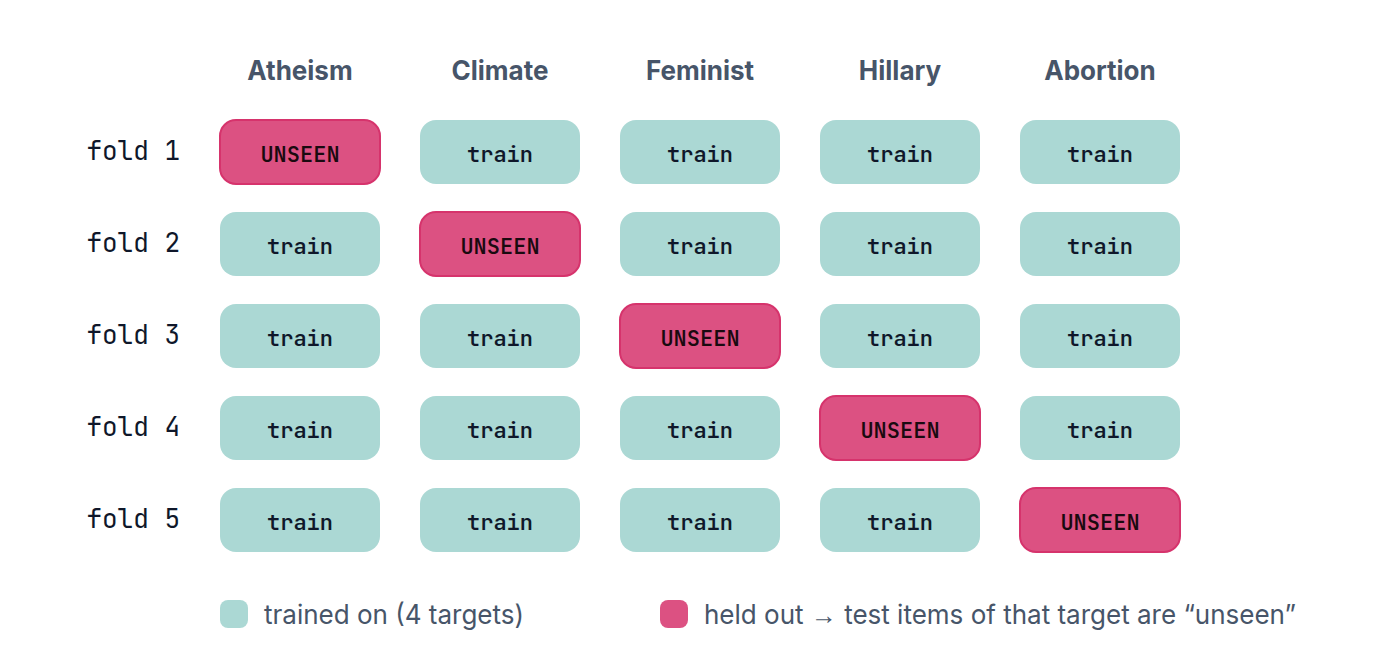
\includegraphics[width=0.6\textwidth]{results/fig/arch/loto.png}
\caption{Leave-one-target-out protocol. Each fold trains on four SemEval targets and holds one out; the official test items of the held-out target are the ``unseen'' items for that fold.}
\label{fig:loto}
\end{figure}

\textbf{Protocol.} AdamW $2\times10^{-5}$, 5 epochs, batch 32, max length 128, bf16 autocast with fp32 master weights; $M=5$ members (seed $i$ + 80\% bootstrap); MC-dropout $T=10$; CreNet $\delta=0.5$; CreDRO $\delta_i\in\{0.5,0.625,0.75,0.875,1\}$. Leave-one-target-out (LOTO): five folds, each excluding one SemEval target from training; the official test set is then split into seen and unseen items. 151 member trainings ($\approx$45\,s each) on one RTX PRO 5000; all credal, conformal and decision computations on CPU from cached outputs.
\textbf{Metrics.} Accuracy, $F_{avg}$ (official: mean F1 of \textsc{favor} and \textsc{against}), macro-F1, ECE (15 bins), NLL; misclassification AUROC and AURC with TU \cite{geifman2017}; unseen-target AUROC with EU, width and TU; determinacy, set accuracy, $u_{65}$ \cite{zaffalon2012}; Spearman $\rho$ between AU/EU/TU and human entropy; JSD/TV between $p^*$ and $\lambda_x$; conformal coverage/efficiency over 100 random 50/50 re-splits of the voted cal$\,\cup\,$test items; expected decision cost with $c_{err}=1$, $c_{defer}=0.3$, $c_{set}=0.15$ per extra class. ``TU'' is the upper entropy for credal methods and the predictive entropy otherwise; ``EU'' is $\up H-\lo H$ for credal methods, mutual information for DE/MCD, vacuity for EDL \cite{sensoy2018} and $1-\max p$ for single models.

% =====================================================================
\section{Results}
% =====================================================================

\subsection{E1: In-target accuracy, calibration and selective prediction}

\begin{table}[h]
\centering\footnotesize\setlength{\tabcolsep}{3.5pt}
\begin{tabular}{l ccc cc cc ccc c}
\toprule
Method & Acc & $F_{avg}$ & mF1 & ECE & NLL & AUROC-err & AURC & Determ. & Set acc & $u_{65}$ & width \\
\midrule
Softmax & 0.742 & 0.756 & 0.718 & 0.154 & 0.696 & \best{0.789} & 0.103 & -- & -- & -- & -- \\
TempScale \cite{guo2017} & 0.742 & 0.756 & 0.718 & 0.077 & 0.590 & 0.785 & 0.104 & -- & -- & -- & -- \\
MCD-MI & 0.757 & 0.771 & 0.729 & 0.087 & 0.583 & 0.754 & 0.105 & -- & -- & -- & -- \\
MCD-Credal & 0.755 & 0.766 & 0.725 & 0.050 & \best{0.571} & 0.741 & 0.110 & 0.676 & 0.886 & 0.759 & 0.678 \\
EDL & 0.718 & 0.733 & 0.698 & 0.088 & 0.702 & 0.786 & 0.116 & -- & -- & -- & -- \\
DE-MI & 0.761 & 0.773 & \best{0.740} & 0.086 & 0.611 & 0.754 & 0.102 & -- & -- & -- & -- \\
CreWrap-DE & 0.754 & 0.769 & 0.727 & 0.066 & 0.607 & 0.746 & 0.109 & 0.698 & 0.869 & 0.757 & 0.620 \\
CreDE & 0.757 & 0.772 & 0.732 & 0.068 & 0.576 & 0.770 & \best{0.100} & 0.985 & 0.765 & 0.760 & 0.031 \\
CreWrap-Soft & 0.758 & 0.772 & 0.736 & \best{0.029} & 0.578 & 0.729 & 0.113 & 0.692 & 0.874 & 0.758 & 0.587 \\
CreDRO & \best{0.762} & \best{0.775} & \best{0.740} & 0.046 & 0.583 & 0.733 & 0.110 & 0.688 & 0.876 & 0.758 & 0.646 \\
CreDRO-Soft & 0.753 & 0.763 & 0.736 & 0.041 & 0.602 & 0.723 & 0.117 & 0.701 & 0.861 & 0.749 & 0.612 \\
EffCre($\alpha{=}0.5$) & 0.747 & 0.761 & 0.724 & 0.144 & 0.685 & 0.777 & 0.104 & 0.970 & 0.761 & 0.751 & 0.081 \\
EffCre($\alpha{=}10^{-6}$) & 0.748 & 0.762 & 0.724 & 0.127 & 0.650 & 0.775 & 0.104 & 0.880 & 0.802 & \best{0.761} & 0.302 \\
LLM-single (Qwen2.5-3B) & 0.635 & 0.630 & 0.580 & 0.274 & 2.063 & 0.655 & 0.258 & -- & -- & -- & -- \\
LLM-promptMI & 0.632 & 0.628 & 0.581 & 0.215 & 1.651 & 0.647 & 0.262 & -- & -- & -- & -- \\
LLM-PromptCredal & 0.620 & 0.627 & 0.578 & 0.143 & 1.500 & 0.621 & 0.279 & 0.535 & 0.810 & 0.618 & 0.995 \\
\bottomrule
\end{tabular}
\caption{In-target results on the SemEval-2016 test set ($n=1{,}249$). Bootstrap 95\% CIs (1{,}000 resamples): ECE Softmax 0.154 [0.130, 0.177], DE-MI 0.091 [0.071, 0.112], CreWrap-DE 0.072 [0.054, 0.093], CreDRO 0.054 [0.036, 0.072], CreDRO-Soft 0.051 [0.035, 0.069], CreWrap-Soft 0.038 [0.023, 0.054]; AURC Softmax 0.102 [0.087, 0.120] vs CreDRO-Soft 0.118 [0.101, 0.135]; accuracy CIs overlap for all supervised methods.}
\label{tab:e1}
\end{table}

Accuracy is unchanged across supervised methods (overlapping CIs); the official $F_{avg}$ of 0.756--0.775 is in the range reported for BERT-family models on this benchmark \cite{garg2024}. \textbf{Calibration improves monotonically with the amount of credal and soft structure}: 0.154 (softmax) $\to$ 0.077 (temperature) $\to$ 0.066 (credal wrapper) $\to$ 0.046 (DRO) $\to$ 0.029 (soft labels); the soft-label gain has non-overlapping CIs with every hard-label method. \textbf{Selective prediction in-target is not improved}: softmax entropy remains the best error detector (AUROC 0.789) and AURC differences lie within CIs, because credal total uncertainty is deliberately high on contested items that the models often get right. Wrapper-based credal sets abstain to a 2--3-class set on $\approx$30\% of items and are then right 87\% of the time ($u_{65}\approx0.76$). CreDE and EffCre produce very narrow intervals (width 0.03--0.3), consistent with the ``intervals too tight'' observation of \cite{credro2026}.

\subsection{E4a: Unseen-target detection, leave-one-target-out}

\begin{table}[h]
\centering\footnotesize\setlength{\tabcolsep}{3.5pt}
\begin{tabular}{l ccc cc c cc}
\toprule
Method & AUROC (EU) & AUROC (width) & AUROC (TU) & Acc unseen & $F_{avg}$ unseen & AURC unseen & AU seen$\to$unseen & EU seen$\to$unseen \\
\midrule
Softmax & 0.786$\pm$0.052 & 0.786$\pm$0.052 & 0.816$\pm$0.065 & 0.572$\pm$0.135 & 0.511$\pm$0.124 & 0.339$\pm$0.129 & 0.56$\to$1.04 & 0.15$\to$0.31 \\
TempScale & 0.795$\pm$0.055 & 0.795$\pm$0.055 & 0.828$\pm$0.065 & 0.572$\pm$0.135 & 0.511$\pm$0.124 & 0.341$\pm$0.129 & 0.79$\to$1.22 & 0.21$\to$0.38 \\
DE-MI & 0.743$\pm$0.051 & 0.743$\pm$0.051 & 0.875$\pm$0.037 & 0.501$\pm$0.106 & 0.442$\pm$0.121 & 0.439$\pm$0.110 & 0.58$\to$1.05 & 0.12$\to$0.22 \\
CreWrap-DE & 0.623$\pm$0.051 & 0.767$\pm$0.040 & 0.871$\pm$0.042 & 0.506$\pm$0.092 & 0.453$\pm$0.113 & 0.494$\pm$0.087 & 0.28$\to$0.65 & 0.68$\to$0.85 \\
CreDE & 0.520$\pm$0.101 & \best{0.878$\pm$0.039} & 0.890$\pm$0.033 & 0.562$\pm$0.106 & 0.501$\pm$0.119 & 0.390$\pm$0.107 & 0.73$\to$1.24 & 0.05$\to$0.05 \\
CreWrap-Soft & 0.505$\pm$0.043 & 0.760$\pm$0.033 & 0.878$\pm$0.034 & 0.528$\pm$0.087 & 0.477$\pm$0.102 & 0.448$\pm$0.089 & 0.53$\to$0.98 & 0.53$\to$0.54 \\
CreDRO & 0.542$\pm$0.082 & 0.787$\pm$0.025 & 0.897$\pm$0.016 & 0.503$\pm$0.130 & 0.445$\pm$0.146 & 0.469$\pm$0.140 & 0.37$\to$0.75 & 0.72$\to$0.76 \\
\textbf{CreDRO-Soft} & 0.337$\pm$0.106 & 0.759$\pm$0.058 & \best{0.905$\pm$0.021} & 0.523$\pm$0.083 & 0.476$\pm$0.108 & 0.428$\pm$0.087 & 0.64$\to$1.06 & 0.60$\to$0.48 \\
EffCre($\alpha{=}10^{-6}$) & 0.692$\pm$0.045 & 0.810$\pm$0.076 & 0.828$\pm$0.078 & 0.563$\pm$0.130 & 0.502$\pm$0.122 & 0.369$\pm$0.125 & 0.36$\to$0.72 & 0.44$\to$0.60 \\
\bottomrule
\end{tabular}
\caption{Leave-one-target-out: AUROC for separating test tweets of the held-out target from those of seen targets (mean$\pm$std over 5 folds), accuracy on the held-out target, and the mean aleatoric/epistemic scores on seen vs unseen items.}
\label{tab:e4a}
\end{table}

Per-fold unseen AUROC (TU) for CreDRO-Soft: Atheism 0.908, Climate 0.938, Feminism 0.873, Clinton 0.902, Abortion 0.902 (Softmax 0.814/0.916/0.763/0.733/0.854). Paired tests over folds: CreDRO-Soft $>$ Softmax in 5/5 folds ($+0.089$, paired $t$ $p=0.025$); $>$ DE-MI in 4/5 ($+0.030$, $p=0.16$); $>$ CreDRO in 4/5 ($+0.008$, n.s.).

The \textbf{upper entropy of a credal set is the best and most stable unseen-target detector}: 0.905$\pm$0.021 (CreDRO-Soft) and 0.897$\pm$0.016 (CreDRO) against 0.816$\pm$0.065 for softmax entropy and 0.875$\pm$0.037 for the ensemble entropy, with 3--4$\times$ smaller fold-to-fold variance. \textbf{The additive entropy decomposition breaks on unseen targets}: every member becomes nearly uniform on a new target, so the \emph{lower} entropy jumps (0.64$\to$1.06 bits of a maximum 1.585) and $\up H-\lo H$ \emph{shrinks} (0.60$\to$0.48); the EU score becomes anti-correlated with novelty (AUROC 0.34). This is the ``AU saturates, EU has no room'' pathology of entropy-based decompositions discussed by Wimmer et al.\ \cite{wimmer2023}; interval width does not suffer from it (0.76--0.88) and the trained-interval CreDE width is the best epistemic score (0.878); Figure~\ref{fig:eu}. Unseen-target \emph{accuracy} collapses for every method (0.50--0.57 vs 0.73--0.79 on seen targets), which is why detection and deferral matter.

\begin{figure}[h]
\centering
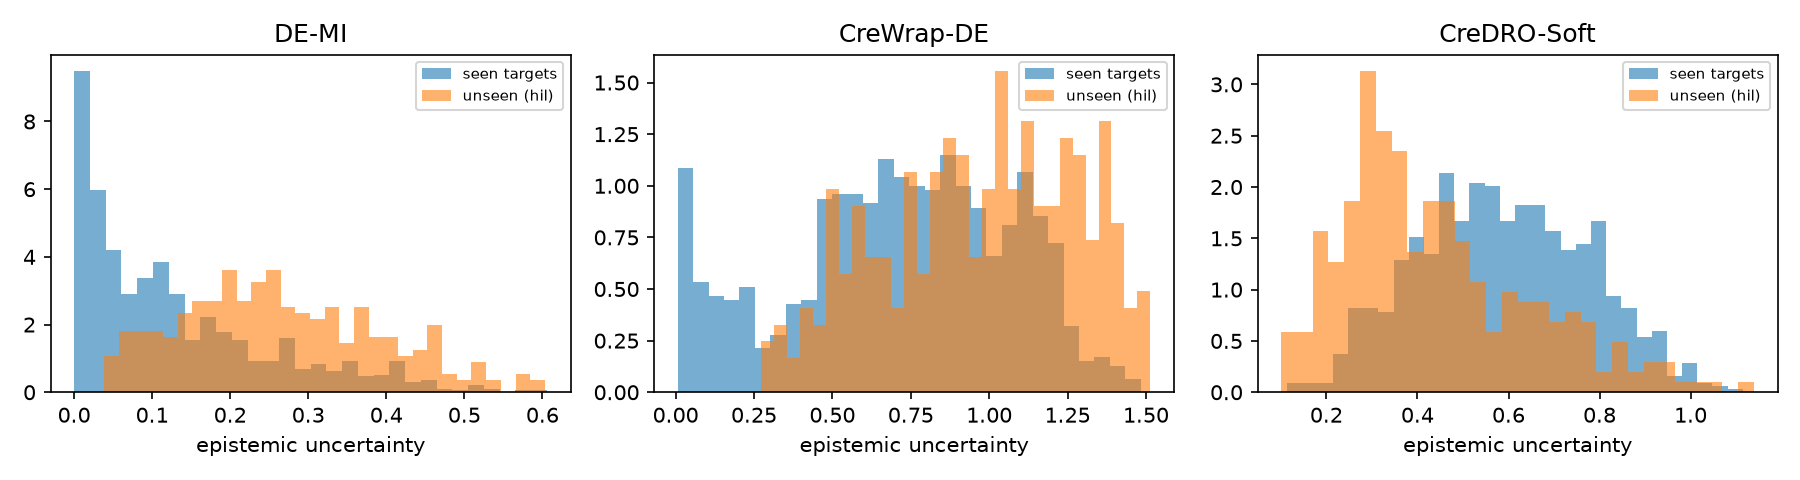
\includegraphics[width=\textwidth]{results/fig/eu_seen_vs_unseen.png}
\caption{Entropy-based epistemic score on seen vs unseen (Clinton) test tweets. For the mutual information (left) and the credal wrapper (middle) the unseen distribution shifts right; for CreDRO-Soft (right) it shifts \emph{left}, because the lower entropy saturates. The width-based score (Table~\ref{tab:e4a}) recovers the expected ordering.}
\label{fig:eu}
\end{figure}

\subsection{E4b: Cross-dataset unseen targets}

\begin{table}[h]
\centering\footnotesize\setlength{\tabcolsep}{3.5pt}
\begin{tabular}{l ccc c ccc cc}
\toprule
 & \multicolumn{4}{c}{P-Stance (political tweets)} & \multicolumn{5}{c}{COVID-19-Stance (health tweets)} \\
\cmidrule(lr){2-5}\cmidrule(lr){6-10}
Method & AUROC EU & width & TU & Acc & AUROC EU & width & TU & Acc & mF1 \\
\midrule
Softmax & 0.594 & 0.594 & 0.597 & 0.724 & 0.874 & 0.874 & 0.895 & 0.585 & 0.586 \\
TempScale & 0.596 & 0.596 & 0.602 & 0.724 & 0.885 & 0.885 & \best{0.910} & 0.585 & 0.586 \\
MCD-MI & 0.450 & 0.450 & 0.519 & 0.674 & 0.535 & 0.535 & 0.846 & 0.554 & 0.557 \\
EDL & 0.539 & 0.539 & 0.551 & 0.673 & 0.763 & 0.763 & 0.808 & 0.554 & 0.544 \\
DE-MI & 0.646 & 0.646 & 0.657 & 0.710 & 0.708 & 0.708 & 0.856 & 0.600 & 0.598 \\
CreWrap-DE & \best{0.651} & 0.641 & 0.680 & 0.681 & 0.671 & 0.737 & 0.867 & 0.595 & 0.596 \\
CreDE & 0.627 & 0.642 & 0.655 & 0.726 & 0.716 & \best{0.902} & 0.848 & 0.609 & \best{0.610} \\
CreWrap-Soft & 0.629 & \best{0.664} & \best{0.713} & 0.712 & 0.501 & 0.730 & 0.877 & \best{0.610} & 0.609 \\
CreDRO & 0.615 & 0.627 & 0.678 & 0.690 & 0.651 & 0.751 & 0.867 & 0.583 & 0.583 \\
CreDRO-Soft & 0.437 & 0.624 & 0.711 & 0.707 & 0.398 & 0.749 & 0.888 & 0.579 & 0.579 \\
EffCre($\alpha{=}10^{-6}$) & 0.579 & 0.592 & 0.597 & 0.713 & 0.790 & 0.890 & 0.904 & 0.585 & 0.588 \\
LLM-PromptCredal & 0.463 & 0.444 & 0.458 & \best{0.744} & 0.481 & 0.475 & 0.475 & 0.532 & 0.517 \\
\bottomrule
\end{tabular}
\caption{SemEval-trained models applied to P-Stance and COVID-19 test tweets: AUROC for separating them from SemEval test tweets, and zero-shot transfer accuracy (P-Stance is binary: the \textsc{none} column is dropped for the argmax).}
\label{tab:e4b}
\end{table}

COVID tweets are far from the training targets and every supervised method detects them with TU (0.85--0.91); P-Stance tweets are political like SemEval and much harder to tell apart (0.60--0.71; best CreWrap-Soft 0.713 and CreDRO-Soft 0.711). The LLM's prompt disagreement carries no information about \emph{our} training distribution (AUROC $<0.5$), as expected: epistemic uncertainty is relative to what a model was trained on.

\subsection{E5: Alignment with human disagreement}

\begin{table}[h]
\centering\small
\begin{tabular}{l ccc cc}
\toprule
Method & $\rho(\AU,H)$ & $\rho(\EU,H)$ & $\rho(\TU,H)$ & JSD$(p^*,\lambda)$ & TV$(p^*,\lambda)$ \\
\midrule
Softmax & 0.318 & 0.311 & 0.318 & 0.162 & 0.289 \\
TempScale & 0.323 & 0.315 & 0.323 & 0.133 & 0.267 \\
MCD-MI & 0.334 & 0.321 & 0.341 & 0.133 & 0.263 \\
EDL & 0.318 & 0.327 & 0.318 & 0.155 & 0.295 \\
DE-MI & 0.325 & 0.277 & 0.321 & 0.144 & 0.271 \\
CreWrap-DE & 0.324 & 0.258 & 0.316 & 0.142 & 0.274 \\
CreDE & 0.327 & 0.106 & 0.327 & 0.136 & 0.265 \\
CreWrap-Soft & \best{0.345} & 0.169 & 0.334 & \best{0.124} & \best{0.260} \\
CreDRO & 0.302 & 0.214 & 0.289 & 0.138 & 0.270 \\
CreDRO-Soft & 0.304 & \best{0.068} & 0.319 & 0.129 & 0.266 \\
EffCre($\alpha{=}10^{-6}$) & 0.317 & 0.323 & 0.328 & 0.149 & 0.279 \\
LLM-PromptCredal & 0.082 & 0.140 & 0.145 & 0.209 & 0.348 \\
\bottomrule
\end{tabular}
\caption{Spearman correlation between predicted uncertainty and human label entropy $H(\lambda_x)$, and divergence between the point prediction and $\lambda_x$, on the 1{,}080 voted test tweets. All $\rho(\AU,H)$ for supervised models have $p<10^{-20}$.}
\label{tab:e5}
\end{table}

Soft-label training gives the best match to human disagreement ($\rho=0.345$, lowest JSD). More important is \emph{discriminant validity}: for credal methods the epistemic score is almost uncorrelated with human entropy ($\rho(\EU,H)=0.07$ for CreDRO-Soft, 0.11 for CreDE, 0.17 for CreWrap-Soft) while the aleatoric score correlates at 0.30--0.35, i.e.\ the two parts of the set carry different information. For a single softmax (and EffCre, which only dilates it) both scores are the same ranking, so no separation is possible. The zero-shot LLM's uncertainty barely tracks human disagreement ($\rho\approx0.1$).

\subsection{E5b: Ambiguity stress test}

\begin{table}[h]
\centering\small
\begin{tabular}{l ccc cc}
\toprule
Method & AUROC (AU) & AUROC (EU) & AUROC (TU) & AU test$\to$ambig & EU test$\to$ambig \\
\midrule
Softmax & 0.652 & 0.648 & 0.652 & 0.45$\to$0.65 & 0.11$\to$0.18 \\
DE-MI & 0.660 & 0.619 & 0.656 & 0.50$\to$0.68 & 0.12$\to$0.16 \\
CreWrap-DE & 0.652 & 0.597 & 0.648 & 0.25$\to$0.36 & 0.60$\to$0.73 \\
CreDE & 0.663 & 0.530 & 0.664 & 0.66$\to$0.88 & 0.04$\to$0.04 \\
CreWrap-Soft & \best{0.668} & 0.521 & 0.653 & 0.55$\to$0.73 & 0.54$\to$0.56 \\
CreDRO & 0.638 & 0.589 & 0.652 & 0.30$\to$0.42 & 0.63$\to$0.72 \\
CreDRO-Soft & 0.653 & \best{0.486} & 0.652 & 0.65$\to$0.81 & 0.54$\to$0.54 \\
EffCre($\alpha{=}10^{-6}$) & 0.648 & 0.636 & 0.654 & 0.28$\to$0.42 & 0.38$\to$0.49 \\
LLM-PromptCredal & 0.578 & 0.575 & 0.578 & 0.04$\to$0.06 & 0.73$\to$0.86 \\
\bottomrule
\end{tabular}
\caption{Separating the 1{,}101 low-agreement tweets (seen targets) from the test set, and the mean scores on each.}
\label{tab:e5b}
\end{table}

Tweets that humans could not agree on are only moderately separable from the test set by any single score (AUROC 0.64--0.67): many \emph{test} tweets are also contested (mean human entropy 0.63 bits). The decisive observation is the \emph{pattern}: for the soft-label methods the aleatoric score rises on the ambiguous pool (0.65$\to$0.81) while the epistemic score stays flat (0.54$\to$0.54; AUROC 0.49--0.52, chance), whereas for the hard-label wrapper both rise together (EU 0.60$\to$0.73). Soft-label supervision is what stops ``contested'' from leaking into ``unknown'' (Figure~\ref{fig:map}).

\begin{figure}[h]
\centering
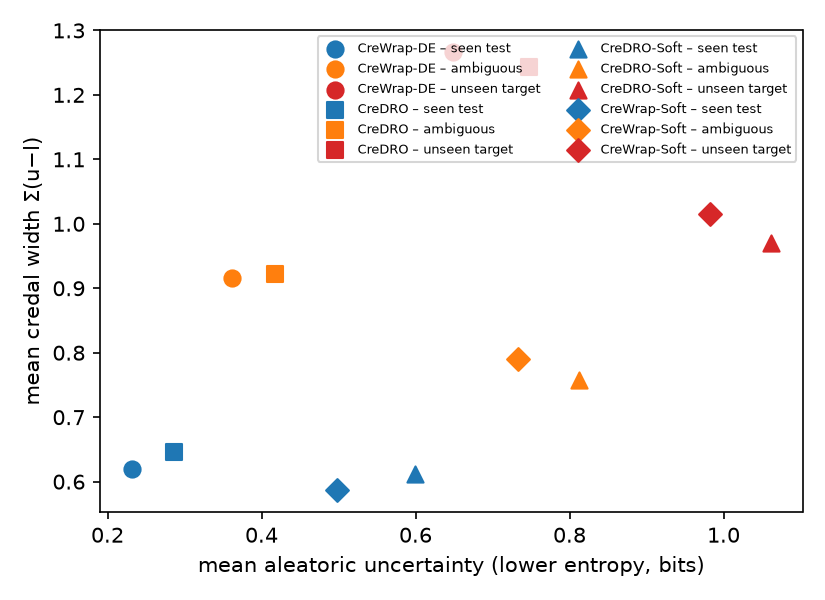
\includegraphics[width=0.62\textwidth]{results/fig/au_eu_map.png}
\caption{Mean aleatoric score vs mean credal width for each credal method on seen test tweets (blue), human-contested tweets (orange) and unseen-target tweets (red, LOTO average). Ambiguity moves points right; novelty moves them up and right.}
\label{fig:map}
\end{figure}

\subsection{E6: Conformal coverage of the human label distribution}

\begin{table}[h]
\centering\small\setlength{\tabcolsep}{4pt}
\begin{tabular}{l ccc ccc ccc}
\toprule
 & \multicolumn{3}{c}{TV ball, $1-\alpha=0.9$} & \multicolumn{3}{c}{TV ball, $1-\alpha=0.8$} & \multicolumn{3}{c}{credal dilation, 0.9} \\
\cmidrule(lr){2-4}\cmidrule(lr){5-7}\cmidrule(lr){8-10}
Method & cov & $\hat q$ & $|\ND|$ & cov & $\hat q$ & $|\ND|$ & cov & $\hat q$ & $|\ND|$ \\
\midrule
Softmax & 0.903 & 0.724 & 3.00 & 0.799 & 0.546 & 2.98 & -- & -- & -- \\
TempScale & 0.903 & 0.642 & 3.00 & 0.798 & 0.478 & 2.92 & -- & -- & -- \\
DE-MI & 0.902 & 0.635 & 3.00 & 0.798 & 0.472 & 2.50 & -- & -- & -- \\
CreWrap-DE & 0.901 & 0.602 & 3.00 & 0.798 & 0.466 & 2.46 & 0.901 & 0.473 & 2.66 \\
CreDE & 0.900 & 0.617 & 3.00 & 0.798 & 0.449 & \best{2.38} & 0.900 & 0.609 & 3.00 \\
CreWrap-Soft & 0.901 & 0.546 & 3.00 & 0.797 & \best{0.436} & 2.58 & 0.900 & 0.420 & 2.64 \\
CreDRO & 0.901 & 0.586 & 3.00 & 0.797 & 0.458 & 2.56 & 0.901 & 0.445 & 2.68 \\
CreDRO-Soft & 0.900 & \best{0.542} & 3.00 & 0.799 & 0.444 & 2.89 & 0.900 & \best{0.416} & 2.90 \\
EffCre($\alpha{=}10^{-6}$) & 0.903 & 0.698 & 3.00 & 0.799 & 0.517 & 2.89 & 0.902 & 0.596 & 3.00 \\
LLM-PromptCredal & 0.899 & 0.757 & 3.00 & 0.799 & 0.598 & 3.00 & 0.900 & 0.705 & 3.00 \\
\bottomrule
\end{tabular}
\caption{Conformal credal sets over 100 random 50/50 re-splits of the 1{,}565 voted cal$\,\cup\,$test items: empirical coverage, calibrated radius and mean number of non-dominated classes.}
\label{tab:e6}
\end{table}

The guarantee holds for every predictor (0.90/0.80 at the nominal levels). Efficiency differs: the radius needed for 90\% coverage falls from 0.724 (softmax) to 0.542 (CreDRO-Soft) and 0.546 (CreWrap-Soft): \textbf{soft-label training produces the most efficient conformal credal sets}. At 90\% the radius is still so large that every class stays non-dominated, because with a median of 8 votes $\lambda_x$ is itself noisy (standard error up to 0.18 per class) and a distribution-free guarantee must be loose; at 80\% the sets become informative (2.4--2.6 classes). The credal-dilation variant needs a smaller additive radius (0.416) because the model's own box already covers part of the discrepancy.

\subsection{E7: Decision value}

\begin{table}[h]
\centering\small
\begin{tabular}{l cccc cccc}
\toprule
 & \multicolumn{4}{c}{confidence thresholding, deferral budget} & \multicolumn{4}{c}{credal routing, deferral budget} \\
\cmidrule(lr){2-5}\cmidrule(lr){6-9}
Method & 0\% & 5\% & 10\% & 20\% & 0\% & 5\% & 10\% & 20\% \\
\midrule
Softmax & 0.258 & 0.242 & 0.228 & 0.213 & -- & -- & -- & -- \\
DE-MI & 0.239 & 0.223 & 0.220 & 0.202 & -- & -- & -- & -- \\
CreWrap-DE & 0.246 & 0.233 & 0.222 & 0.212 & 0.185 & 0.190 & 0.196 & 0.200 \\
CreDE & 0.243 & 0.232 & 0.222 & 0.202 & 0.238 & 0.237 & 0.235 & 0.236 \\
CreWrap-Soft & 0.242 & 0.233 & 0.228 & 0.217 & 0.182 & 0.190 & 0.199 & 0.214 \\
CreDRO & 0.238 & 0.228 & 0.220 & 0.208 & \best{0.181} & \best{0.184} & \best{0.189} & \best{0.197} \\
CreDRO-Soft & 0.247 & 0.241 & 0.236 & 0.218 & 0.194 & 0.200 & 0.210 & 0.223 \\
EffCre($\alpha{=}10^{-6}$) & 0.252 & 0.239 & 0.231 & 0.213 & 0.218 & 0.213 & 0.206 & 0.203 \\
\bottomrule
\end{tabular}
\caption{Expected cost per item on the in-target test set ($c_{err}=1$, $c_{defer}=0.3$, $c_{set}=0.15$ per extra class).}
\label{tab:e7}
\end{table}

Set-valued credal routing lowers the expected cost by about a quarter in-target (0.181 vs 0.238--0.258) \emph{without any deferral}, because interval dominance turns most would-be errors into a cheap two-class answer. On unseen targets (LOTO folds, 10\% deferral budget) the gap widens to 30--50\%: CreDRO 0.246/0.310/0.345/0.283/0.304 vs confidence 0.407/0.685/0.444/0.341/0.512; CreDRO-Soft 0.259/0.278/0.352/0.254/0.332 vs 0.448/0.555/0.436/0.345/0.509; softmax (confidence only) 0.353/0.324/0.398/0.294/0.673. Narrow-interval methods (CreDE, EffCre) gain little because they are almost always determinate.

\subsection{E8: LLM prompt-credal}
Single-prompt accuracy varies from 0.52 to 0.63 across paraphrases; the credal set over prompts halves ECE (0.274$\to$0.143) and reduces NLL (2.06$\to$1.50) at unchanged accuracy, but prompts disagree so much that only 53\% of items receive a single-class answer (width 0.995), and the LLM's uncertainty neither detects our unseen datasets nor tracks human disagreement. Fine-tuned 184M-parameter encoders beat the zero-shot 3B LLM by 12 accuracy points in-target. H5 is supported for calibration only.

\subsection{Ensemble-size ablation}

\begin{table}[h]
\centering\small
\begin{tabular}{l l cccc}
\toprule
Method & Metric & $M=1$ & $M=2$ & $M=3$ & $M=5$ \\
\midrule
CreWrap-DE & ECE / LOTO AUROC (TU) & 0.154 / 0.816 & 0.126 / 0.835 & 0.109 / 0.854 & 0.066 / 0.871 \\
CreDRO & ECE / LOTO AUROC (TU) & 0.093 / 0.877 & 0.076 / 0.888 & 0.070 / \best{0.906} & 0.046 / 0.897 \\
CreDRO-Soft & ECE / LOTO AUROC (TU) & 0.066 / 0.888 & 0.045 / 0.910 & 0.047 / \best{0.919} & 0.041 / 0.905 \\
CreWrap-Soft & ECE / LOTO AUROC (TU) & 0.077 / 0.843 & 0.059 / 0.857 & 0.052 / 0.875 & \best{0.029} / 0.878 \\
\bottomrule
\end{tabular}
\caption{Effect of ensemble size (first $M$ members). A single soft-label DRO model already beats a five-member hard-label ensemble on both calibration and unseen-target detection; width-based scores need $M\ge2$ and saturate at $M=3$. Extending the in-target ensembles to $M=8$ brings no further gain (ECE 0.064/0.046/0.045/0.025 for the four rows; COVID unseen AUROC (TU) 0.859/0.864/0.881/0.879) while the mean width keeps growing (0.69--0.78), so $M=5$ is used for every main table.}
\label{tab:abl}
\end{table}

% =====================================================================
\section{Discussion}
% =====================================================================

\paragraph{What the credal representation buys for stance.} Three things, each measured: (1) calibrated class probabilities without a post-hoc temperature (ECE 0.03--0.05 vs 0.15), (2) the most stable unseen-target detector in the study (upper entropy, 0.90$\pm$0.02 vs 0.82$\pm$0.07 for softmax entropy), and (3) a set-valued answer that cuts decision cost by $\approx$25\% in-target and 30--50\% on unseen targets without deferring anything. It does \emph{not} buy a better in-target error detector: softmax entropy remains best there (H1 holds for calibration, not for selective risk).

\paragraph{Which construction.} Post-hoc wrapping of a deep ensemble is the baseline; replacing seed diversity by DRO diversity (CreDRO) improves calibration and unseen-target AUROC at identical cost; replacing hard labels by human label distributions (Soft) improves calibration further, gives the best human alignment and the most efficient conformal sets, and keeps the epistemic score flat on ambiguous items. Combining both (CreDRO-Soft) gives the best unseen-target detection and the cleanest ambiguity/novelty separation, at the price of slightly higher in-target AURC. Trained-interval heads (CreDE) give excellent width-based novelty detection but near-degenerate sets; EffCre is the cheapest option and matches softmax-level novelty detection on COVID but cannot separate the two kinds of uncertainty.

\paragraph{A measurement result.} The textbook decomposition $\EU=\up H-\lo H$ is unusable for unseen-target detection in three-class stance: members collapse to near-uniform predictions on a new target, the lower entropy saturates and the difference shrinks. Interval width (or the distance-based measures of \cite{gonzalez2026}) should be used for the epistemic part and the upper entropy for total uncertainty. Figure~\ref{fig:eupath} illustrates the mechanism.

\begin{figure}[t]
\centering
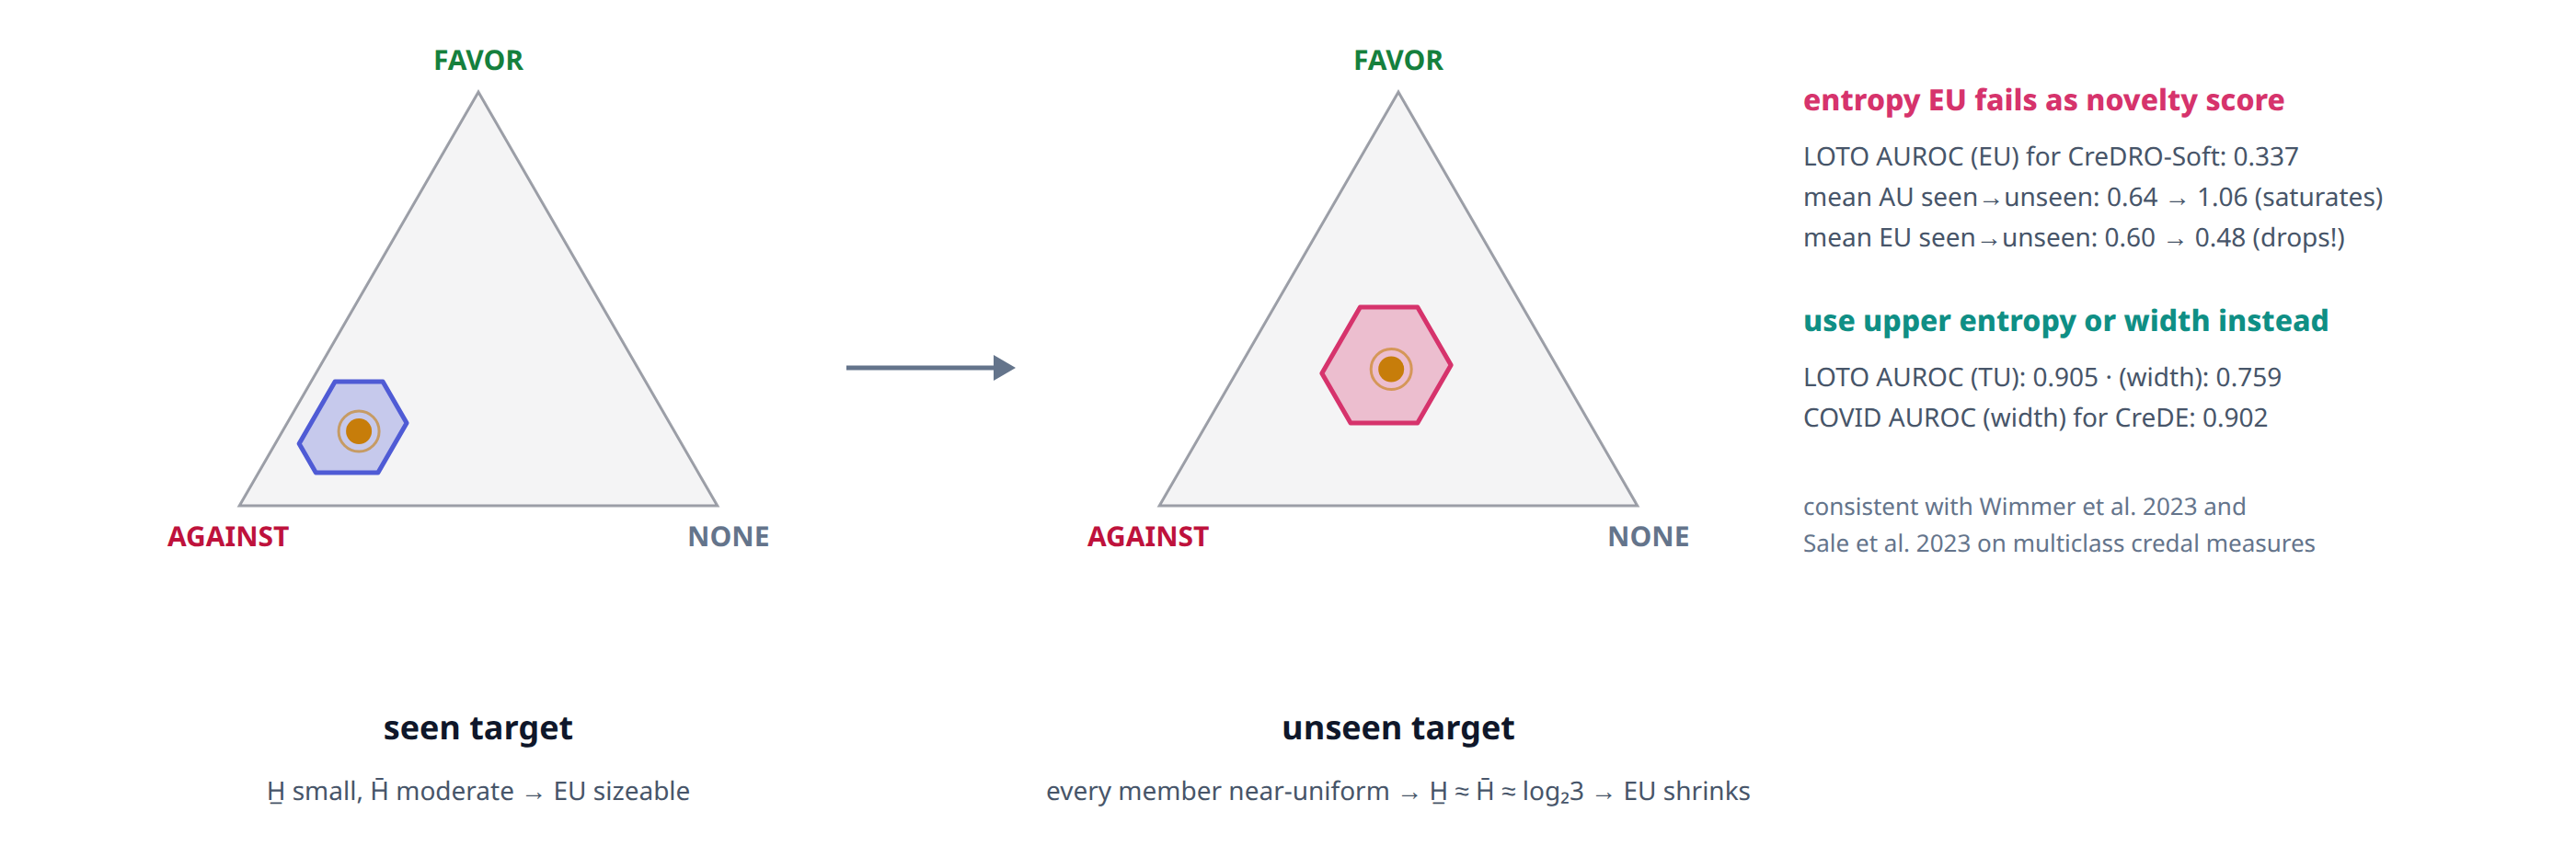
\includegraphics[width=\textwidth]{results/fig/arch/eu_pathology.png}
\caption{Why the entropy-based epistemic score fails on unseen targets. On a seen target members are confident: $\lo H$ is small and $\up H-\lo H$ is sizeable. On an unseen target every member collapses towards uniform, $\lo H$ saturates near $\log_2 3$ and the difference shrinks although the box itself is larger. Upper entropy or width should be used instead.}
\label{fig:eupath}
\end{figure}

\paragraph{Human label distributions with 8 votes.} They are informative enough to train on and to calibrate on, but too noisy for a 90\% distribution-free guarantee to be tight; ChaosNLI-style data with $\sim$100 votes \cite{nie2020} would close that gap.

\section{Limitations}
One backbone size and $M=5$; human votes exist only for four SemEval targets, so human-alignment claims are scoped to SemEval; conformal guarantees assume exchangeability and do not transfer across datasets; LLM experiments are zero-shot (no LoRA-ensemble credal LLMs); unseen-target accuracy is low for every method ($\approx$0.5): this work improves \emph{knowing} when the model is out of its depth, not the stance prediction itself.

\section{Conclusion}
We built and evaluated six ways of giving a stance detector a credal output and proposed one that combines distributional robustness with supervision from publicly available per-annotator votes. On SemEval-2016, P-Stance and COVID-19-Stance the proposal calibrates as well as the best method in the study, detects unseen targets with the highest and most stable AUROC (0.905$\pm$0.021; 5/5 folds over softmax, $p=0.025$), is the only family whose epistemic score stays flat on human-contested tweets, yields the most efficient conformal credal sets, and reduces expected decision cost by 25--50\% through set-valued answers. We also showed that the standard entropy-based epistemic measure is unsuitable for this task and that a single soft-label DRO model is a strong, cheap alternative. No new annotation was needed; all code, cached outputs and tables are reproducible from the repository.

% =====================================================================
\begin{thebibliography}{99}\small

\bibitem{abellan2006} J.~Abell\'an, G.~J. Klir, S.~Moral. Disaggregated total uncertainty measure for credal sets. \emph{Int.\ J.\ General Systems}, 35(1):29--44, 2006.
\bibitem{allaway2020} E.~Allaway, K.~McKeown. Zero-shot stance detection: A dataset and model using generalized topic representations. \emph{EMNLP}, 2020.
\bibitem{angelopoulos2023} A.~N. Angelopoulos, S.~Bates. Conformal prediction: A gentle introduction. \emph{Found.\ Trends ML}, 16(4), 2023.
\bibitem{corani2008} G.~Corani, M.~Zaffalon. Learning reliable classifiers from small or incomplete data sets: The naive credal classifier 2. \emph{JMLR}, 9:581--621, 2008.
\bibitem{cozman2000} F.~G. Cozman. Credal networks. \emph{Artificial Intelligence}, 120(2):199--233, 2000.
\bibitem{credro2026} Learning credal ensembles via distributionally robust optimization. \emph{arXiv:2602.08470}, 2026.
\bibitem{gal2016} Y.~Gal, Z.~Ghahramani. Dropout as a Bayesian approximation. \emph{ICML}, 2016.
\bibitem{garg2024} K.~Garg, C.~Caragea. Stanceformer: Target-aware transformer for stance detection. \emph{Findings of EMNLP}, 2024.
\bibitem{geifman2017} Y.~Geifman, R.~El-Yaniv. Selective classification for deep neural networks. \emph{NeurIPS}, 2017.
\bibitem{glandt2021} K.~Glandt, S.~Khanal, Y.~Li, D.~Caragea, C.~Caragea. Stance detection in COVID-19 tweets. \emph{ACL}, 2021.
\bibitem{gonzalez2026} X.~Gonzalez-Garcia, S.~L. Chau, J.~Rodemann, M.~Caprio, K.~Muandet, H.~Bustince, S.~Destercke, E.~H\"ullermeier, Y.~Sale. Quantification of credal uncertainty: A distance-based approach. \emph{arXiv:2603.27270}, 2026.
\bibitem{guo2017} C.~Guo, G.~Pleiss, Y.~Sun, K.~Q. Weinberger. On calibration of modern neural networks. \emph{ICML}, 2017.
\bibitem{he2023} P.~He, J.~Gao, W.~Chen. DeBERTaV3. \emph{ICLR}, 2023.
\bibitem{hofman2026} P.~Hofman, T.~L\"ohr, M.~Muschalik, Y.~Sale, E.~H\"ullermeier. Efficient credal prediction through decalibration. \emph{ICLR}, 2026.
\bibitem{hullermeier2021} E.~H\"ullermeier, W.~Waegeman. Aleatoric and epistemic uncertainty in machine learning. \emph{Machine Learning}, 110:457--506, 2021.
\bibitem{javanmardi2024} A.~Javanmardi, D.~Stutz, E.~H\"ullermeier. Conformalized credal set predictors. \emph{NeurIPS}, 2024.
\bibitem{kucuk2020} D.~K\"u\c{c}\"uk, F.~Can. Stance detection: A survey. \emph{ACM Computing Surveys}, 53(1), 2020.
\bibitem{lakshminarayanan2017} B.~Lakshminarayanan, A.~Pritzel, C.~Blundell. Simple and scalable predictive uncertainty estimation using deep ensembles. \emph{NeurIPS}, 2017.
\bibitem{li2021} Y.~Li, T.~Sosea, A.~Sawant, A.~J. Nair, D.~Inkpen, C.~Caragea. P-Stance: A large dataset for stance detection in political domain. \emph{Findings of ACL}, 2021.
\bibitem{lohr2025} T.~L\"ohr, P.~Hofman, F.~Mohr, E.~H\"ullermeier. Credal prediction based on relative likelihood. \emph{NeurIPS}, 2025.
\bibitem{manchingal2026} S.~Kudukkil Manchingal, S.~Nikolenko, F.~Cuzzolin. Credal large language models for semantic commitment under uncertainty. \emph{arXiv:2608.23244}, 2026.
\bibitem{mohammad2016} S.~M. Mohammad, S.~Kiritchenko, P.~Sobhani, X.~Zhu, C.~Cherry. SemEval-2016 Task 6: Detecting stance in tweets. \emph{SemEval}, 2016.
\bibitem{mohammad2017} S.~M. Mohammad, P.~Sobhani, S.~Kiritchenko. Stance and sentiment in tweets. \emph{ACM TOIT}, 17(3), 2017. Raw annotations: \url{https://saifmohammad.com/WebPages/StanceDataset.htm}.
\bibitem{nie2020} Y.~Nie, X.~Zhou, M.~Bansal. What can we learn from collective human opinions on natural language inference data? \emph{EMNLP}, 2020.
\bibitem{sale2023} Y.~Sale, M.~Caprio, E.~H\"ullermeier. Is the volume of a credal set a good measure for epistemic uncertainty? \emph{UAI}, 2023.
\bibitem{sensoy2018} M.~Sensoy, L.~Kaplan, M.~Kandemir. Evidential deep learning to quantify classification uncertainty. \emph{NeurIPS}, 2018.
\bibitem{troffaes2007} M.~C.~M. Troffaes. Decision making under uncertainty using imprecise probabilities. \emph{IJAR}, 45(1):17--29, 2007.
\bibitem{walley1991} P.~Walley. \emph{Statistical Reasoning with Imprecise Probabilities}. Chapman \& Hall, 1991.
\bibitem{wang2024crede} K.~Wang, F.~Cuzzolin, S.~Kudukkil Manchingal, K.~Shariatmadar, D.~Moens, H.~Hallez. Credal deep ensembles for uncertainty quantification. \emph{NeurIPS}, 2024.
\bibitem{wang2025wrapper} K.~Wang, F.~Cuzzolin, et~al. Credal wrapper of model averaging for uncertainty estimation in classification. \emph{ICLR}, 2025.
\bibitem{wang2025creinn} K.~Wang et~al. CreINNs: Credal-set interval neural networks for uncertainty estimation in classification tasks. \emph{Neural Networks}, 2025.
\bibitem{wimmer2023} L.~Wimmer, Y.~Sale, P.~Hofman, B.~Bischl, E.~H\"ullermeier. Quantifying aleatoric and epistemic uncertainty in machine learning: Are conditional entropy and mutual information appropriate measures? \emph{UAI}, 2023.
\bibitem{xiong2024} M.~Xiong et~al. Can LLMs express their uncertainty? An empirical evaluation of confidence elicitation in LLMs. \emph{ICLR}, 2024.
\bibitem{zaffalon2012} M.~Zaffalon, G.~Corani, D.~Mau\'a. Evaluating credal classifiers by utility-discounted predictive accuracy. \emph{IJAR}, 53(8):1282--1301, 2012.
\bibitem{zhao2024} C.~Zhao, C.~Caragea. EZ-STANCE: A large dataset for English zero-shot stance detection. \emph{ACL}, 2024.
\end{thebibliography}

\end{document}
